\chapter{Cơ sở Lý thuyết}
    \section{Tổng quan về Lĩnh vực}
        \subsection{Khái niệm Internet vạn vật (IoT)}
            Internet vạn vật (Internet of Things – IoT) là một mô hình kết nối các đối tượng vật lý, thiết bị và cảm biến với Internet, cho phép chúng thu thập, trao đổi và phân tích dữ liệu mà không cần sự can thiệp trực tiếp từ con người. IoT tạo ra một mạng lưới các thiết bị không đồng nhất như thiết bị gia dụng, máy móc công nghiệp và cảm biến, có khả năng giao tiếp với nhau thông qua nhiều giao thức và tiêu chuẩn khác nhau.

            Trong bối cảnh phát triển công nghệ hiện nay, hệ thống IoT đóng vai trò ngày càng quan trọng trong các lĩnh vực khác nhau, từ nhà thông minh, thành phố thông minh, công nghiệp 4.0, cho đến nông nghiệp dữ liệu. Sự đa dạng của các thiết bị và giao thức truyền thông tạo ra nhu cầu cấp thiết cho các giải pháp trung gian có khả năng tích hợp và quản lý hiệu quả.

            % \begin{figure}[H]
            %     \centering
            %     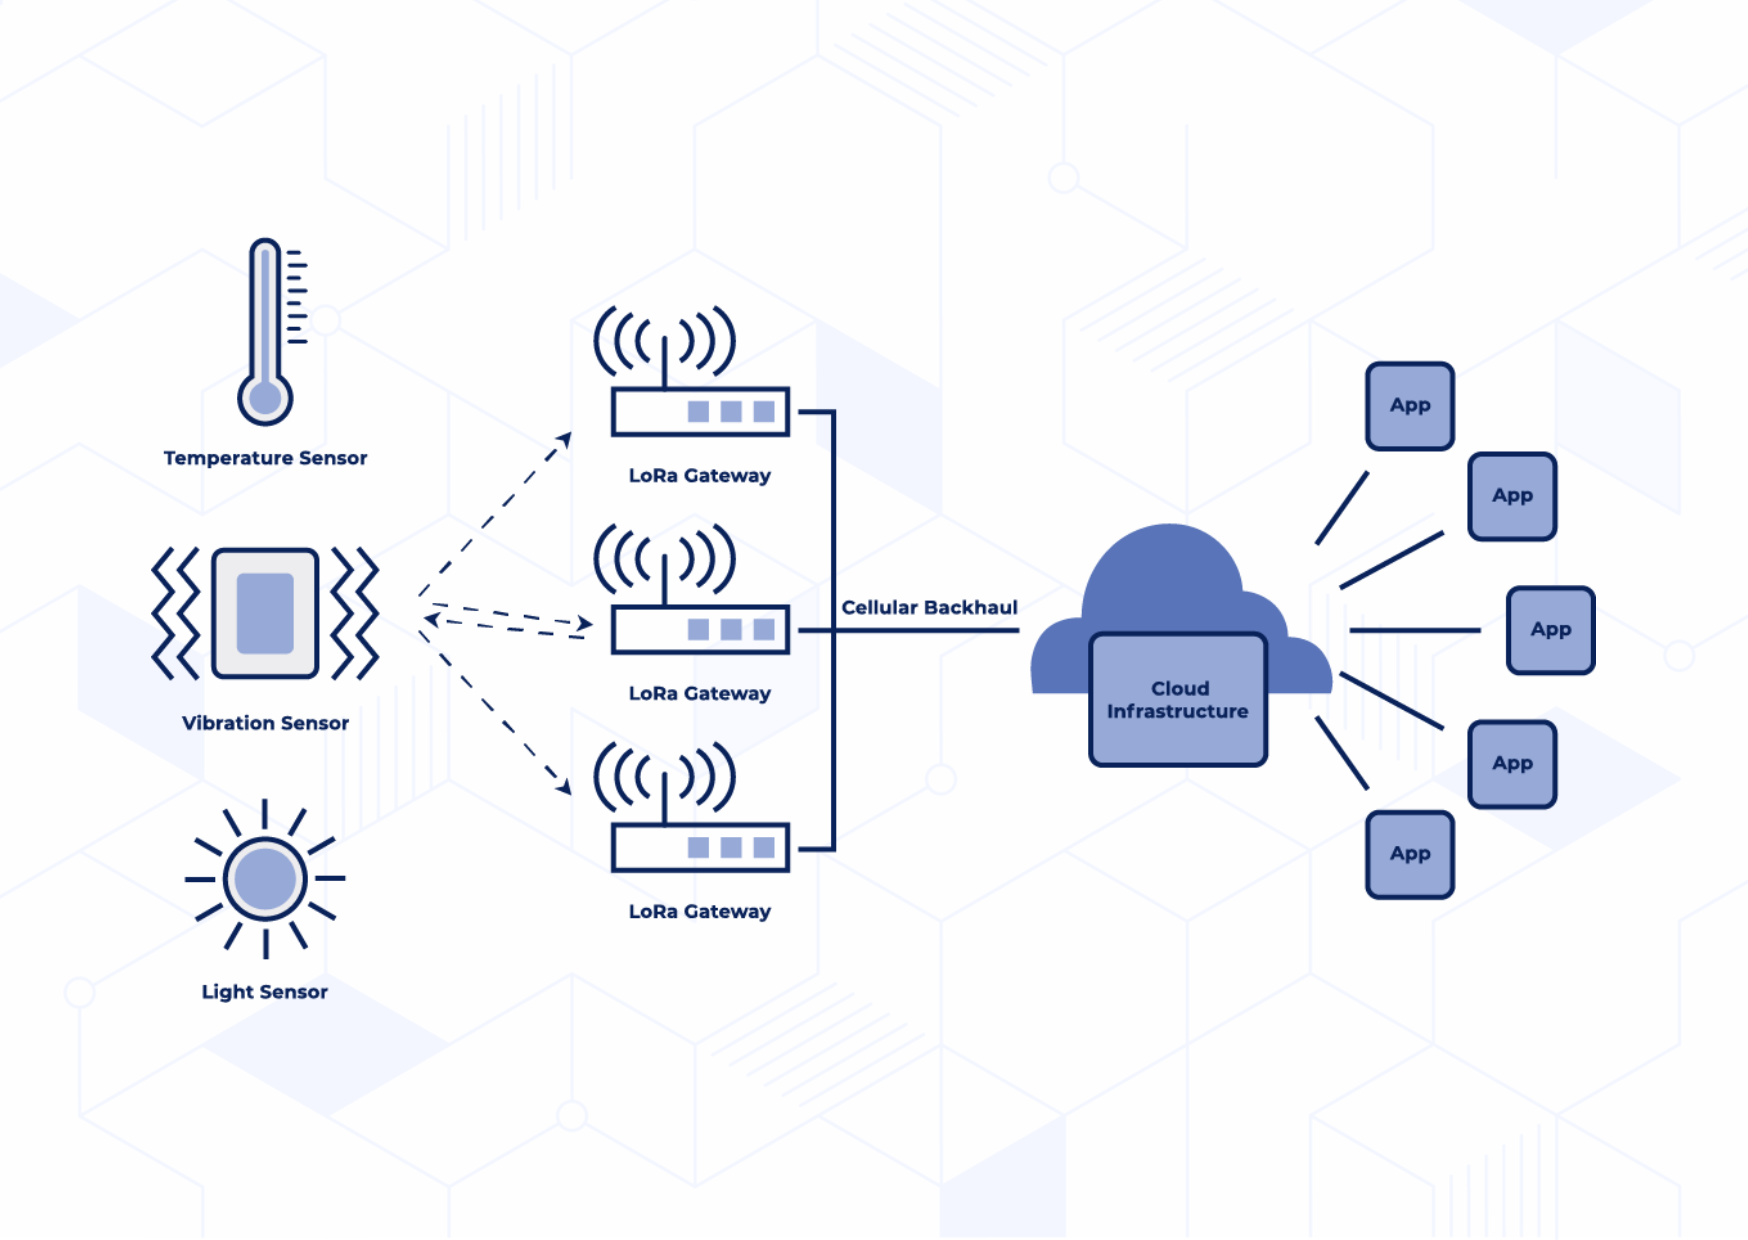
\includegraphics[width=0.7\textwidth]{figures/iot_network.png}
            %     \vspace{1em}
            %     \caption{Hạ tầng Internet vạn vật (IoT)}
            %     \label{fig:iot_overview}
            % \end{figure}

        \subsection{Vị trí và vai trò của IoT gateway}
            IoT gateway đóng vai trò như một cầu nối quan trọng giữa các thiết bị IoT và các nền tảng đám mây, hoạt động như một trung tâm điều phối chính, cho phép truyền thông và luồng dữ liệu trong hạ tầng Internet vạn vật. Gateway là thành phần then chốt giữa lớp cảm nhận (perception layer), gồm các cảm biến và thiết bị và lớp mạng (network layer) kết nối đến các dịch vụ đám mây.

            Theo tiêu chuẩn công nghiệp, một gateway IoT được định nghĩa là một thiết bị phần cứng hoặc ứng dụng phần mềm đóng vai trò là điểm kết nối giữa máy chủ ứng dụng IoT và các thiết bị đầu cuối. Tiêu chuẩn ITU-T Y.4418 định nghĩa gateway là "một đơn vị trong Internet vạn vật có chức năng kết nối các thiết bị với mạng truyền thông, thực hiện việc chuyển đổi cần thiết giữa các giao thức được sử dụng trong mạng truyền thông và các giao thức mà thiết bị sử dụng."

            IoT gateway hoạt động như những trung tâm thông minh, liên kết các thiết bị IoT và đám mây với nhau, đảm nhiệm việc chuyển đổi giao tiếp giữa các thiết bị IoT cũng như lọc và xử lý dữ liệu thành thông tin hữu ích. Chúng tạo ra cầu nối giữa các cảm biến và cơ cấu chấp hành (actuators) ở một phía, và các nền tảng hậu kỳ (quản lý dữ liệu, thiết bị và người dùng) ở phía còn lại.
    \section{Cơ sở lý thuyết về IoT Gateway}
        \subsection{Khái niệm IoT gateway}
            IoT gateway trong lĩnh vực Internet of Things đóng vai trò là nút trung gian giữa các mạng cảm biến và nền tảng đám mây hoặc trung tâm dữ liệu được kết nối thông qua Internet. Mục tiêu chính của gateway là xử lý tính không đồng nhất do các thiết bị và giao thức khác nhau tạo ra, thu thập lượng lớn dữ liệu ở nhiều định dạng khác nhau và chuyển tiếp dữ liệu đã xử lý lên các hệ thống mức cao hơn.

            Để hệ thống IoT vận hành và được quản lý đúng cách, dữ liệu thu thập từ thiết bị biên cần được làm sạch, tiền xử lý và lọc trước khi gửi đến trung tâm dữ liệu, tuỳ theo yêu cầu của từng ứng dụng. IoT gateway được thiết kế để đảm nhiệm những chức năng này một cách hiệu quả tại biên mạng.

            Về mặt chức năng, IoT gateway có thể được hiểu thông qua ba năng lực cốt lõi:
            \begin{enumerate}
                \item \textbf{Chuyển tiếp thông điệp (Message Forwarding):} khả năng truyền tải dữ liệu giữa các thiết bị và hệ thống xử lý tập trung một cách đáng tin cậy, bảo toàn ngữ nghĩa và chất lượng dịch vụ (QoS) mong muốn.
                \item \textbf{Xử lý cục bộ (Local Processing):} thực hiện các tác vụ điện toán biên (edge computing) để xử lý, tổng hợp hoặc ra quyết định tại chỗ, giúp giảm độ trễ, tiết kiệm băng thông và giảm phụ thuộc vào kết nối liên tục với cloud.
                \item \textbf{Khả năng mở rộng tài nguyên (Resource Openness):} cung cấp các giao diện và dịch vụ chung cho nhiều ứng dụng IoT, cho phép quản lý thiết bị, phát hiện và truy cập các tài nguyên (sensors, actuators, dữ liệu, \dots) một cách thống nhất.
            \end{enumerate}

            Nhờ ba năng lực trên, IoT gateway không chỉ đóng vai trò là điểm trung chuyển dữ liệu mà còn là một nút điện toán biên thông minh, giúp giảm độ trễ, tối ưu băng thông và hỗ trợ ra quyết định gần thời gian thực ngay tại biên mạng.

        \subsection{Vị trí của IoT gateway trong kiến trúc IoT}
            IoT gateway chiếm vị trí chiến lược trong kiến trúc nhiều lớp của hệ thống IoT. Theo tiêu chuẩn của IEEE, trong ba lớp của Internet vạn vật (gồm lớp cảm nhận, lớp mạng và lớp ứng dụng), gateway là thành phần thiết yếu vì lớp cảm nhận và lớp mạng thuộc về các mạng dị thể (heterogeneous networks) vốn không thể giao tiếp trực tiếp với nhau.

            Các IoT gateway đóng vai trò là liên kết trung gian, cho phép thông tin thu thập từ các cảm biến IoT được chuyển đổi và đóng gói thành các gói dữ liệu mạng để truyền đến các máy chủ backend hoặc nền tảng đám mây. Nhờ đó, IoT gateway trở thành điểm then chốt trong việc đảm bảo luồng dữ liệu ổn định và tin cậy trong toàn bộ hạ tầng IoT.

            Trong bối cảnh phân cấp mạng IoT, các IoT gateway hoạt động như các điểm hội tụ dữ liệu (aggregation points), nơi nhiều thiết bị IoT hợp nhất luồng dữ liệu của chúng trước khi truyền lên các hệ thống cấp cao hơn. Vị trí chiến lược này cho phép IoT gateway quản lý và tối ưu hóa luồng dữ liệu từ nhiều thiết bị đầu cuối, đảm bảo sử dụng băng thông hiệu quả và giảm tải xử lý cho hạ tầng đám mây.
            \begin{figure}[h]
                \centering
                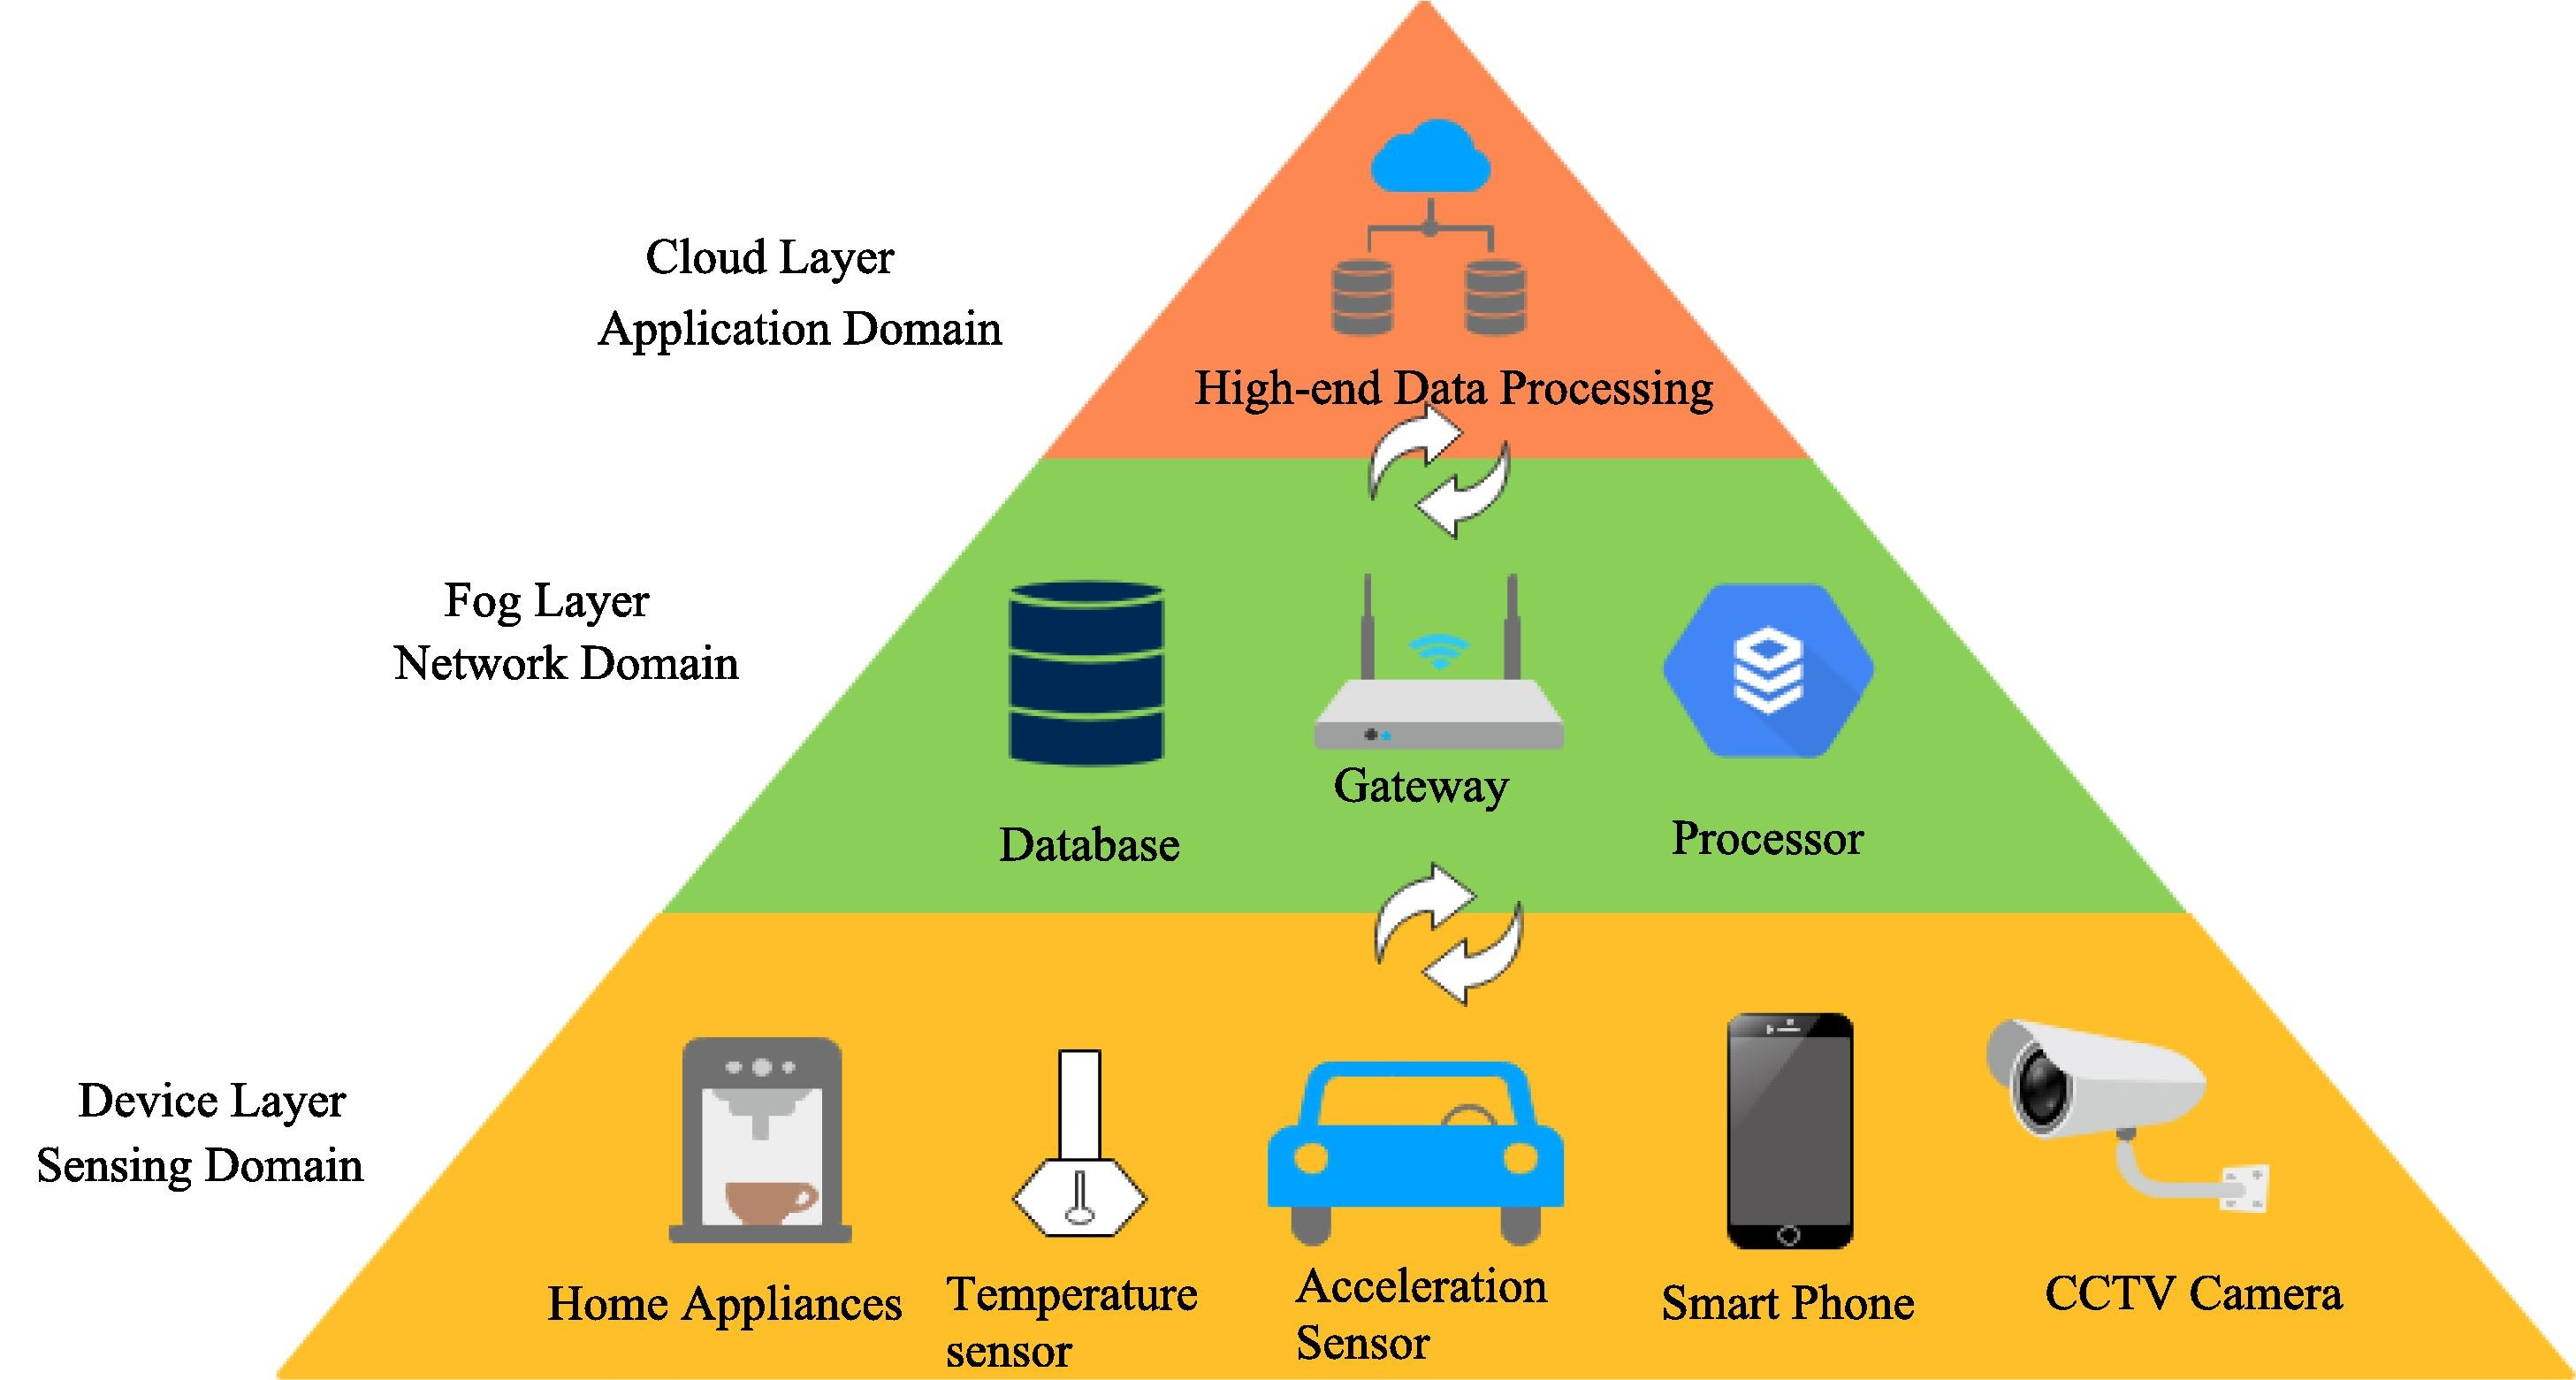
\includegraphics[width=0.7\textwidth]{figures/Gateway_in_IoT_architecture.jpg}
                \vspace{1em}
                \caption{Vị trí của IoT gateway trong kiến trúc IoT}
                \label{fig:iot_gateway_position}
            \end{figure}
        \subsection{Các vai trò chính của IoT gateway}
            IoT Gateway không chỉ là một điểm kết nối đơn thuần mà là một hệ thống đa chức năng: tổng hợp dữ liệu từ nhiều thiết bị đầu cuối, chuyển đổi giao thức không đồng nhất, thực thi bảo mật, và xử lý dữ liệu tại biên. Các vai trò này phối hợp chặt chẽ để giúp IoT gateway trở thành thành phần trọng tâm của bất kỳ kiến trúc IoT hiệu quả.
                \subsubsection*{Tổng hợp và quản lý dữ liệu (data aggregation and management)}
                    IoT gateway thu thập dữ liệu từ nhiều thiết bị và cảm biến IoT, hợp nhất các luồng thông tin trước khi chuyển tiếp đến các nền tảng đám mây hoặc trung tâm dữ liệu. Chức năng tổng hợp này giúp giảm lưu lượng mạng và cho phép xử lý dữ liệu hiệu quả hơn. Gateway có thể thực hiện các hoạt động như lọc dữ liệu trùng lặp, phân loại theo loại hoặc nguồn, và tính toán các chỉ số tổng hợp.

                \subsubsection*{Chuyển đổi giao thức (protocol translation)}
                    Một trong những chức năng quan trọng nhất của IoT gateway là khả năng chuyển đổi hai chiều giữa các giao thức truyền thông khác nhau. Thiết bị có thể chuyển dữ liệu từ các giao thức công nghiệp cũ như Modbus sang các giao thức IoT hiện đại như MQTT hoặc HTTP, giúp tích hợp liền mạch giữa hạ tầng hiện có và hệ thống IoT mới. Khả năng này rất cần thiết để xây dựng một kiến trúc truyền thông thống nhất trong môi trường thiết bị không đồng nhất.

                \subsubsection*{Khả năng điện toán biên (edge computing capabilities)}
                    Các IoT gateway hiện đại ngày càng tích hợp chức năng điện toán biên, cho phép xử lý và phân tích dữ liệu tại chỗ mà không cần phụ thuộc hoàn toàn vào kết nối đám mây. Cách tiếp cận xử lý phân tán này giúp phản hồi theo thời gian thực đối với các sự kiện quan trọng, giảm tải, giảm độ trễ cho các hệ thống xử lý trung tâm và tiết kiệm băng thông. Điểm toán biên cho phép thực hiện các tác vụ như phát hiện bất thường, cảnh báo ngưỡng vượt, hoặc ra quyết định tác động nhanh chóng.

                \subsubsection*{Thực thi bảo mật (security enforcement)}
                    IoT gateway thường được xem như lớp phòng tuyến bảo mật đầu tiên của hạ tầng IoT. Thông qua gateway, các cơ chế như kiểm soát truy cập, xác thực và phân quyền thiết bị/người dùng, mã hóa dữ liệu (ví dụ: TLS/DTLS, VPN) và lọc gói (firewall, ACL) được triển khai tập trung ở một điểm. Gateway đóng vai trò điểm thực thi chính sách bảo mật (policy enforcement point), kiểm tra và áp dụng các quy tắc đối với cả lưu lượng từ thiết bị lên cloud (uplink) lẫn từ cloud về thiết bị (downlink). Bên cạnh đó, gateway có thể tích hợp các chức năng phát hiện bất thường, ghi nhật ký truy vết (audit log) và quản lý chứng chỉ số, giúp phục vụ công tác giám sát, phân tích sự cố và đảm bảo tuân thủ các yêu cầu an toàn thông tin của hệ thống.

                \subsubsection*{Quản lý kết nối và thiết bị (connectivity and device management)}
                    IoT gateway không chỉ duy trì kết nối mạng cho các thiết bị đầu cuối mà còn đóng vai trò nền tảng quản lý thiết bị tập trung. Thông qua gateway, hệ thống có thể giám sát trạng thái kết nối, chất lượng liên kết, cấu hình tham số hoạt động và điều khiển thiết bị từ xa. Gateway thường hỗ trợ các chức năng như tự động phát hiện (device discovery), đăng ký/huỷ đăng ký thiết bị, cập nhật firmware qua mạng (FOTA) và chẩn đoán lỗi từ xa. Việc tập trung các chức năng này tại gateway giúp đơn giản hóa công tác vận hành, giảm tải cho nền tảng cloud và cho phép quản trị viên quản lý toàn bộ hệ sinh thái IoT một cách thống nhất, hiệu quả.

                \subsubsection*{Lưu trữ cục bộ và bộ nhớ đệm (local storage and caching)}
                    Nhiều IoT gateway cung cấp khả năng lưu trữ tạm thời, cho phép lưu đệm dữ liệu trong trường hợp mất kết nối và đồng bộ lại khi kết nối được khôi phục. Tính năng này giúp đảm bảo tính liên tục và toàn vẹn của dữ liệu trong các môi trường có kết nối mạng không ổn định. Bộ nhớ đệm cho phép gateway tiếp tục hoạt động độc lập trong một khoảng thời gian nhất định ngay cả khi kết nối với cloud bị ngắt.
        \subsection{Cấu trúc của IoT gateway}
            Một IoT Gateway hiện đại được thiết kế theo kiến trúc nhiều lớp (layered architecture), trong đó mỗi lớp đảm nhận một nhóm chức năng cụ thể và phối hợp chặt chẽ với các lớp khác. Cấu trúc này không chỉ tạo ra sự tách biệt rõ ràng giữa phần cứng và phần mềm, mà còn cho phép gateway hoạt động như một nền tảng tính toán linh hoạt, có thể mở rộng và dễ bảo trì. Về tổng thể, kiến trúc của gateway có thể chia thành hai khối chính: khối phần cứng (hardware layer) đảm nhiệm việc thu nhận và truyền dẫn tín hiệu vật lý, và khối phần mềm nhiều lớp (multi-layer software stack) thực hiện các chức năng xử lý, quản lý và giao tiếp cấp cao.
            \begin{figure}[h]
                \centering
                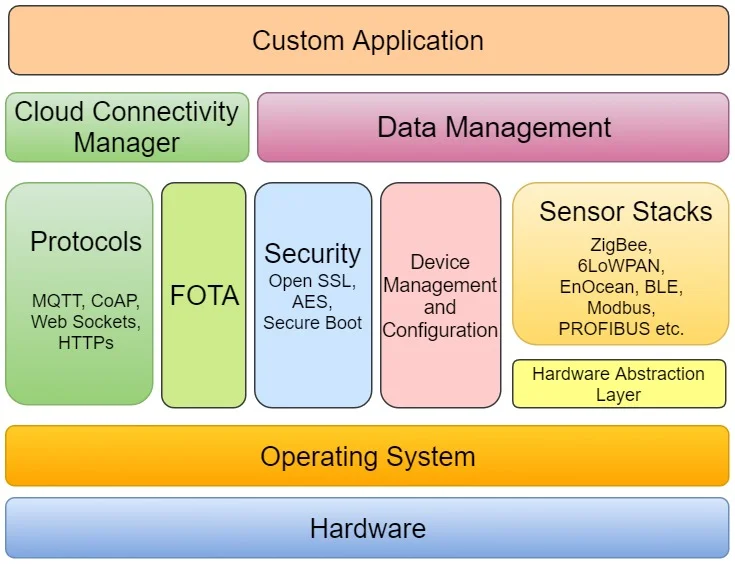
\includegraphics[width=0.7\textwidth]{figures/iot_gateway_architecture.png}
                \vspace{1em}
                \caption{Cấu trúc của IoT gateway}
                \label{fig:iot_gateway_structure}
            \end{figure}
                \subsubsection{Kiến trúc phần cứng}
                    Lớp phần cứng là nền tảng vật lý của gateway, cung cấp khả năng kết nối, tính toán và lưu trữ cần thiết cho toàn bộ hệ thống. Các thành phần chính của kiến trúc phần cứng bao gồm:

                    \textbf{Bộ xử lý trung tâm và bộ nhớ} \\
                        Gateway sử dụng vi xử lý hoặc vi điều khiển có năng lực xử lý đủ mạnh kết hợp với bộ nhớ RAM và bộ nhớ Flash/eMMC để lưu trữ hệ điều hành, firmware và dữ liệu tạm thời. Tùy vào yêu cầu ứng dụng, gateway có thể sử dụng Single Board Computer (SBC) như Raspberry Pi, hoặc các nền tảng công nghiệp chuyên dụng có khả năng hoạt động trong môi trường khắc nghiệt.

                    \textbf{Các mô-đun giao tiếp và kết nối} \\
                        Đây là thành phần cốt lõi giúp gateway kết nối với thiết bị biên và mạng Internet:
                        \begin{itemize}
                            \item Kết nối có dây: Ethernet (Fast Ethernet/Gigabit), RS-232, RS-485/422, Modbus RTU, CAN bus phục vụ giao tiếp với các thiết bị công nghiệp, cảm biến và PLC.
                            \item Kết nối không dây tầm ngắn: Bluetooth Low Energy (BLE), Zigbee, Z-Wave, Wi-Fi (2.4/5 GHz) để kết nối với các thiết bị IoT trong phạm vi cục bộ như cảm biến, công tắc, thiết bị gia dụng thông minh.
                            \item Kết nối không dây tầm xa: LoRa/LoRaWAN, NB-IoT, LTE-M, 4G/5G để truyền dữ liệu lên cloud hoặc server từ xa.
                        \end{itemize}

                    \textbf{Nguồn điện và quản lý năng lượng} \\
                        Khối nguồn DC/DC hoặc AC/DC converter cung cấp nguồn ổn định cho toàn bộ hệ thống, thường hỗ trợ nguồn đầu vào rộng và tích hợp các mạch bảo vệ chống quá áp, quá dòng, chống đảo cực để đảm bảo gateway hoạt động tin cậy trong môi trường công nghiệp. Một số gateway còn hỗ trợ Power over Ethernet (PoE) để giảm thiểu cáp nguồn riêng biệt.

                    \textbf{Khối bảo mật phần cứng}\\
                        Nhiều gateway hiện đại tích hợp thêm các chip bảo mật chuyên dụng như Trusted Platform Module (TPM) hoặc Secure Element. Các phần tử này được dùng để lưu trữ khóa mã hóa, chứng chỉ số và hỗ trợ các cơ chế như Secure Boot, mã hóa bộ nhớ, xác thực thiết bị bằng chứng chỉ X.509, qua đó nâng cao mức độ an toàn bảo mật ngay từ tầng phần cứng.

                    \textbf{Các cổng mở rộng và I/O}\\
                        Gateway thường cung cấp các chân GPIO, ADC/DAC (chuyển đổi tương tự/số), cổng USB, khe cắm thẻ nhớ SD/microSD và khe SIM để mở rộng khả năng kết nối và lưu trữ.

                \subsubsection{Kiến trúc phần mềm}
                    Trên nền tảng phần cứng, kiến trúc phần mềm của gateway được tổ chức thành các lớp chức năng độc lập, tạo thành một hệ thống phân tầng rõ ràng từ lớp phần cứng đến lớp ứng dụng. Các lớp chính bao gồm:

                    \textbf{Lớp hệ điều hành (Operating System)}\\
                        Hệ điều hành cung cấp nền tảng phần mềm cơ bản để quản lý tài nguyên phần cứng, lập lịch tiến trình, quản lý bộ nhớ và cung cấp môi trường thực thi cho các dịch vụ phía trên. Tuỳ yêu cầu, gateway có thể sử dụng RTOS cho các tác vụ thời gian thực hoặc Linux nhúng (OpenWrt, Debian, Ubuntu Core, \dots) cho các ứng dụng phức tạp hỗ trợ container và tích hợp cloud.
                    
                    \textbf{Lớp trừu tượng phần cứng (Hardware Abstraction Layer -- HAL)}\\
                        HAL cung cấp tập API thống nhất để các mô-đun phần mềm tương tác với ngoại vi phần cứng (UART, SPI, I\textsuperscript{2}C, radio, \dots) mà không phụ thuộc vào chi tiết triển khai của từng nền tảng gateway. Điều này giúp tăng tính khả chuyển, cho phép cùng một mã nguồn ứng dụng có thể chạy trên các bo mạch phần cứng khác nhau chỉ bằng cách thay đổi HAL.
                    
                    \textbf{Lớp ngăn xếp cảm biến (Sensor Stacks)}\\
                        Lớp này hiện thực các driver và ngăn xếp giao thức cho mạng cảm biến và thiết bị như ZigBee, 6LoWPAN, EnOcean, BLE, Modbus, PROFIBUS,\dots{} Nó chịu trách nhiệm thu thập dữ liệu từ các nút cảm biến/chấp hành, chuyển về định dạng nội bộ thống nhất để các mô-đun quản lý dữ liệu và ứng dụng có thể sử dụng.
                    
                    \textbf{Lớp giao thức truyền thông (Protocols)}\\
                        Lớp giao thức cung cấp các protocol ở tầng ứng dụng phục vụ trao đổi dữ liệu với cloud hoặc hệ thống bên ngoài, điển hình như MQTT, CoAP, WebSockets, HTTP/HTTPS,\dots{} Các mô-đun này được xây dựng trên nền TCP/UDP của hệ điều hành và được các khối quản lý dữ liệu, quản lý cloud sử dụng để gửi/nhận các gói tin.
                    
                    \textbf{Lớp cập nhật firmware từ xa (FOTA/OTA)}\\
                        Mô-đun FOTA chịu trách nhiệm kiểm tra, tải về, xác thực và cài đặt các bản cập nhật phần mềm/firmware từ cloud. Ngoài việc đảm bảo gateway luôn được vá lỗi và cập nhật tính năng mới, lớp này còn hỗ trợ cơ chế rollback trong trường hợp cập nhật thất bại, giúp hệ thống duy trì trạng thái ổn định.
                    
                    \textbf{Lớp bảo mật (Security)}\\
                        Lớp bảo mật cung cấp các dịch vụ như mã hoá, quản lý khoá và chứng chỉ, thư viện bảo mật (ví dụ TLS/OpenSSL, AES), cũng như cơ chế secure boot và xác thực thiết bị. Các dịch vụ này được các lớp giao thức, FOTA, quản lý thiết bị và ứng dụng sử dụng xuyên suốt để đảm bảo tính bảo mật, toàn vẹn và xác thực của dữ liệu.
                    
                    \textbf{Lớp quản lý và cấu hình thiết bị (Device Management and Configuration)}\\
                        Lớp này quản lý vòng đời của thiết bị IoT: đăng ký/huỷ đăng ký, lưu trữ thuộc tính (kiểu thiết bị, vị trí, tham số hoạt động), giám sát trạng thái, cấu hình tham số, cũng như hỗ trợ cập nhật firmware và chẩn đoán từ xa. Đây là điểm tập trung cho việc quản lý tập trung số lượng lớn node cảm biến/actuator.
                    
                    \textbf{Lớp quản lý dữ liệu (Data Management)}\\
                        Lớp quản lý dữ liệu chịu trách nhiệm tiếp nhận luồng dữ liệu từ sensor stacks, thực hiện lọc, tiền xử lý, tổng hợp và lưu trữ đệm. Mô-đun này giúp giảm băng thông bằng việc chỉ gửi dữ liệu cần thiết, bảo vệ dữ liệu khi kết nối cloud không ổn định (buffering và đồng bộ lại khi có mạng), đồng thời hỗ trợ các chức năng xử lý biên như phát hiện bất thường hoặc áp dụng rule engine.
                    
                    \textbf{Lớp quản lý kết nối cloud (Cloud Connectivity Manager)}\\
                        Cloud Connectivity Manager đảm nhiệm việc thiết lập và duy trì kết nối hai chiều giữa gateway và nền tảng cloud: quản lý phiên làm việc, gửi heartbeat, xử lý cơ chế reconnect, xác thực gateway với cloud và ánh xạ trạng thái thiết bị trên cloud. Lớp này sử dụng các giao thức ở mô-đun \emph{Protocols} và cung cấp API thống nhất cho lớp ứng dụng.
                    
                    \textbf{Lớp ứng dụng tuỳ biến (Custom Application)}\\
                        Trên cùng là lớp ứng dụng tuỳ biến, nơi hiện thực logic nghiệp vụ cụ thể của hệ thống: các kịch bản tự động hoá, xử lý cảnh báo và sự kiện, dashboard cục bộ cho cấu hình/giám sát, cũng như các dịch vụ tích hợp với hệ SCADA/MES/ERP hoặc nền tảng quản lý vận hành khác. Các ứng dụng này tận dụng toàn bộ dịch vụ do các lớp phía dưới cung cấp để xây dựng giải pháp IoT hoàn chỉnh.

        \subsection{Nguyên lý hoạt động cơ bản của IoT Gateway}
            Quá trình hoạt động của gateway là một vòng lặp liên tục: thu thập dữ liệu từ thiết bị đầu cuối, xử lý và lọc tại chỗ, truyền gói tin lên cloud, nhận lệnh điều khiển từ cloud, và gửi lệnh xuống thiết bị. Trong suốt quá trình này, gateway phải đảm bảo tính nhất quán dữ liệu, bảo mật thông tin, phát hiện và xử lý lỗi, cũng như duy trì kết nối liên tục ngay cả trong điều kiện mạng không ổn định. Những yêu cầu này làm cho độ tin cậy, hiệu suất, và bảo mật trở thành những tiêu chí bắt buộc chứ không phải tuỳ chọn trong bất kỳ triển khai thực tế nào.
                \subsubsection*{Thu thập dữ liệu (Data Ingestion)}
                    Gateway tiếp nhận dữ liệu thô từ các cảm biến và thiết bị có cơ cấu chấp hành thông qua các giao thức kết nối được hỗ trợ (như ZigBee, LoRa, BLE, Modbus...). Đây là bước đầu tiên, giúp gateway đóng vai trò là điểm thu gom dữ liệu từ lớp thiết bị (perception layer). Dữ liệu thô này có thể ở các định dạng khác nhau tùy thuộc vào loại cảm biến và giao thức sử dụng.
                \subsubsection*{Xử lý cục bộ (Local Processing)}
                    Trước khi truyền dữ liệu đi, gateway có thể thực hiện các tác vụ xử lý tại chỗ như lọc nhiễu, loại bỏ dữ liệu trùng lặp, tổng hợp số đo, hoặc phát hiện các bất thường thông qua rule engine hoặc thuật toán phân tích biên (edge analytics). Nhờ đó, gateway giúp giảm lưu lượng truyền và tiết kiệm chi phí lưu trữ trên nền tảng đám mây. Các tác vụ xử lý này có thể được cấu hình linh hoạt theo nhu cầu của ứng dụng cụ thể.
                \subsubsection*{Định tuyến giao thức (Protocol Routing)}
                    Gateway mã hóa dữ liệu bằng các giao thức bảo mật trước khi truyền lên nền tảng đám mây, giúp bảo vệ thông tin nhạy cảm trong quá trình di chuyển qua mạng. Trên nền tảng đám mây, dữ liệu tiếp tục được phân tích, trực quan hóa và lưu trữ để tạo ra thông tin chi tiết phục vụ cho việc hình thành hành động hoặc kích hoạt các quy trình tự động. Sau khi xử lý, dữ liệu được định tuyến đến các hệ thống đích phù hợp như dịch vụ đám mây, MQTT broker hoặc cơ sở dữ liệu cục bộ. 
                \subsubsection*{Điều khiển và quản lý từ xa (Remote Control and Management)}
                    Ngoài các nhiệm vụ truyền dữ liệu, gateway cũng nhận các thông tin từ nền tảng đám mây hoặc hệ thống quản lý để gửi lệnh điều khiển xuống các thiết bị biên, cập nhật phần mềm (OTA update), hoặc thay đổi tham số vận hành. Cơ chế này giúp duy trì khả năng quản lý tập trung và đảm bảo thiết bị luôn hoạt động theo đúng cấu hình mong muốn.
                \subsubsection*{Dự phòng và lưu đệm (Failover and Caching)}
                    Trong trường hợp mất kết nối mạng hoặc đám mây, gateway có khả năng lưu trữ tạm thời dữ liệu cục bộ (caching) và đồng bộ lại khi kết nối được phục hồi. Một số gateway còn hỗ trợ tính năng clustering (cụm gateway) để tăng tính sẵn sàng và đảm bảo hoạt động liên tục. Cơ chế này là rất quan trọng đối với các ứng dụng yêu cầu tính tin cậy cao.
                \subsubsection*{Thực thi bảo mật (Security Enforcement)}
                    Gateway là tuyến phòng thủ đầu tiên trong hệ thống IoT, thực hiện các biện pháp bảo mật như mã hóa dữ liệu (encryption), xác thực thiết bị (authentication), và lọc gói tin (packet filtering) để đảm bảo an toàn cho dữ liệu cả trong quá trình truyền và khi lưu trữ. Gateway thực hiện kiểm soát truy cập, ngăn chặn các kết nối trái phép, và giám sát hoạt động để phát hiện các bất thường bảo mật.
    \section{Phân tích các sản phẩm trên thị trường}
        \subsection{Các công nghệ kết nối phổ biến}
            Trong hạ tầng IoT hiện đại, các gateway cần hỗ trợ đa dạng công nghệ kết nối để tích hợp với nhiều loại thiết bị khác nhau. Các công nghệ kết nối tầm ngắn như \textbf{Wi-Fi}, \textbf{Bluetooth Low Energy (BLE)}, \textbf{Zigbee}, \textbf{Z-Wave} được sử dụng rộng rãi trong các ứng dụng gia dụng và văn phòng. Trong khi đó, các công nghệ \textbf{LPWAN} như \textbf{LoRaWAN}, \textbf{NB-IoT}, \textbf{LTE-M} phù hợp với những kịch bản yêu cầu phạm vi phủ sóng rộng và tiêu thụ năng lượng thấp.

            Bên cạnh đó, các kết nối có dây như \textbf{Ethernet}, \textbf{RS-485}, \textbf{RS-232}, \textbf{CAN} vẫn giữ vai trò quan trọng trong môi trường công nghiệp nhờ độ ổn định cao và khả năng chống nhiễu tốt. Việc hỗ trợ đa giao thức kết nối giúp gateway tương thích với hạ tầng thiết bị hiện hữu, đồng thời tạo điều kiện thuận lợi cho việc mở rộng và nâng cấp hệ thống trong tương lai.
        \subsection{Các giao thức truyền dữ liệu}
            Tại tầng ứng dụng, các giao thức truyền dữ liệu phổ biến gồm:
            \begin{itemize}
                \item \textbf{MQTT}: phù hợp nhất cho môi trường hạn chế tài nguyên nhờ mô hình publish--subscribe nhẹ, hỗ trợ cơ chế QoS và hoạt động tốt trên đường truyền không ổn định.
                \item \textbf{CoAP}: được thiết kế cho thiết bị nhẹ, hoạt động trên nền UDP giúp giảm overhead truyền thông, thích hợp cho mạng cảm biến và ứng dụng cần tối giản băng thông.
                \item \textbf{HTTP/HTTPS}: được ưu tiên trong các ứng dụng cần bảo mật cao, dễ tích hợp trực tiếp với hệ thống web, REST API và các dịch vụ cloud truyền thống.
                \item \textbf{AMQP}: hướng tới các hệ thống doanh nghiệp cần hàng đợi thông điệp tin cậy, đảm bảo giao nhận và tích hợp với middleware.
                \item \textbf{XMPP}: phù hợp cho các ứng dụng cần giao tiếp hai chiều theo thời gian gần thực và mô hình nhắn tin mở rộng giữa các nút IoT.
            \end{itemize}
        \subsection{Các mô hình triển khai gateway}
            Trong thực tế, kiến trúc IoT thường áp dụng hai mô hình triển khai gateway chính: mô hình phân tán, trong đó thiết bị đầu cuối đồng thời đảm nhiệm vai trò gateway, và mô hình tập trung với một gateway trung tâm phục vụ nhiều thiết bị đầu cuối.
            
            \subsubsection*{Thiết bị đầu cuối kiêm chức năng gateway (mô hình phân tán)}
                Ở mô hình này, mỗi thiết bị đầu cuối (end device) vừa thực hiện chức năng cảm biến/điều khiển, vừa tích hợp đầy đủ khả năng kết nối mạng và giao tiếp trực tiếp với cloud hoặc server trung tâm (ví dụ: camera IP thông minh, đồng hồ điện thông minh,\dots).
                
                Điều này đòi hỏi bản thân thiết bị:
                \begin{itemize}
                    \item có tài nguyên phần cứng đủ mạnh (CPU, RAM, bộ nhớ lưu trữ) để vận hành hệ điều hành, ngăn xếp giao thức mạng, các cơ chế bảo mật và logic ứng dụng;
                    \item có nguồn năng lượng ổn định (thường là nguồn AC hoặc pin dung lượng lớn) do phải duy trì kết nối mạng và xử lý liên tục.
                \end{itemize}
                
                Ưu điểm của mô hình phân tán là mỗi nút có thể hoạt động độc lập, giảm phụ thuộc vào một gateway trung tâm và nâng cao tính sẵn sàng của hệ thống. Tuy nhiên, khi số lượng thiết bị tăng cao, việc để tất cả nút tự kết nối lên cloud có thể:
                \begin{itemize}
                    \item làm tăng số lượng kết nối và lưu lượng trên mạng backbone, tiềm ẩn nguy cơ nghẽn mạng;
                    \item làm tăng chi phí phần cứng trên từng thiết bị do cần tích hợp thêm tài nguyên xử lý và kết nối;
                    \item khiến công tác quản lý, cập nhật và bảo trì phần mềm trên diện rộng trở nên phức tạp.
                \end{itemize}
            
            \subsubsection*{Nhiều thiết bị đầu cuối kết nối đến một gateway trung tâm (mô hình tập trung)}
                Trong mô hình tập trung, các cảm biến và thiết bị trường chủ yếu thực hiện chức năng đo lường/điều khiển cơ bản, giao tiếp qua các kết nối tầm ngắn hoặc fieldbus (RS-485/Modbus, CAN, Zigbee,\dots) đến một IoT gateway trung tâm. Gateway chịu trách nhiệm:
                \begin{itemize}
                    \item tập trung thu thập, tiền xử lý và tổng hợp dữ liệu;
                    \item chuyển đổi giao thức và quản lý kết nối lên cloud;
                    \item thực thi bảo mật, quản lý thiết bị và hỗ trợ cập nhật phần mềm.
                \end{itemize}
                
                Mô hình này cho phép:
                \begin{itemize}
                    \item đơn giản hoá và giảm chi phí phần cứng của thiết bị đầu cuối, đồng thời giảm yêu cầu về năng lượng tại từng nút;
                    \item hạn chế số lượng kết nối trực tiếp tới cloud, giúp dễ dàng quản lý và giảm nguy cơ nghẽn ở lớp mạng;
                    \item thuận lợi trong việc bảo trì, nâng cấp gateway mà ít ảnh hưởng đến toàn bộ hệ thống cảm biến.
                \end{itemize}
                
                Nhược điểm là gateway trở thành thành phần trọng yếu; nếu không được thiết kế cơ chế dự phòng (redundancy), nó có thể trở thành \emph{điểm lỗi đơn} (single point of failure) của toàn hệ thống.
        \subsection{Các tính năng quan trọng của gateway trên thị trường}
            Các gateway phổ biến hiện nay thường tích hợp những tính năng sau:
            \begin{itemize}
                \item Hỗ trợ đa giao thức kết nối (Wi-Fi, Ethernet, Zigbee, LoRa, BLE, LTE, \ldots)
                \item Chuyển đổi giao thức hai chiều (protocol translation)
                \item Xử lý dữ liệu tại biên (edge computing)
                \item Lưu trữ dữ liệu cục bộ (local storage)
                \item Quản lý và điều khiển thiết bị từ xa
                \item Hỗ trợ cập nhật firmware OTA
                \item Hệ thống bảo mật mạnh: mã hóa, xác thực, kiểm soát truy cập
                \item Hỗ trợ giao diện cấu hình thân thiện
                \item Tích hợp dễ dàng với nền tảng cloud (AWS IoT, Azure IoT, Adafruit IO)
            \end{itemize}
        \subsection{Ví dụ về các gateway thực tế trên thị trường}
            \subsubsection*{M5Stack IoT gateway series}
                M5Stack cung cấp các giải pháp gateway IoT dựa trên nền tảng ESP32 với khả năng kết nối đa dạng (Wi-Fi, BLE, LoRa). Các thiết bị này hỗ trợ giao thức MQTT, HTTP và có thể lập trình dễ dàng thông qua Arduino IDE hoặc MicroPython. M5Stack gateway phù hợp cho các ứng dụng prototyping và phát triển nhanh. Hai dòng sản phẩm tiêu biểu là CoreS3-Lite và CoreMP135.
                \paragraph*{M5Stack CoreS3-Lite}
                    Thiết bị nhỏ gọn của M5Stack với khả năng hoạt động như một mini-gateway hoặc HMI trong hệ thống IoT quy mô nhỏ. Nhờ tích hợp sẵn Wi-Fi/BLE, màn hình cảm ứng, cảm biến và các giao tiếp mở rộng, CoreS3-Lite có thể vừa thu thập dữ liệu, hiển thị trạng thái, vừa giao tiếp với nhiều thiết bị ngoại vi thông qua các mô-đun.
                    \begin{itemize}
                        \item MCU \textbf{ESP32-S3}, lõi kép Xtensa LX7 240\,MHz, hỗ trợ \textbf{Wi-Fi 2.4\,GHz} và \textbf{Bluetooth Low Energy (BLE)}.
                        \item Bộ nhớ \textbf{Flash 16\,MB}, \textbf{PSRAM 8\,MB}, đủ cho ứng dụng có giao diện đồ hoạ, kết nối mạng và xử lý dữ liệu cảm biến.
                        \item Màn hình \textbf{IPS 2.0''} cảm ứng điện dung, độ phân giải 320$\times$240, phù hợp làm giao diện HMI mini (nút bấm, slider, biểu đồ,\dots).
                        \item Tích hợp \textbf{camera 0.3\,MP}, cảm biến ánh sáng/tiệm cận \textbf{LTR-553}, \textbf{IMU 6 trục} và \textbf{từ kế 3 trục}, cho phép xây dựng các ứng dụng nhận diện cơ bản, phát hiện chuyển động, tương tác theo hướng nhìn,\dots
                        \item Khối âm thanh gồm \textbf{codec ES7210}, \textbf{ampli I2S} và \textbf{loa 1\,W} cùng \textbf{micro kép}, hỗ trợ các ứng dụng trợ lý giọng nói, phát cảnh báo âm thanh,\dots
                        \item \textbf{Hỗ trợ GPIO/I\textsuperscript{2}C/UART} thông qua:
                        \begin{itemize}
                            \item Cổng mở rộng dạng HY2.0/Grove trên thân thiết bị để kết nối trực tiếp cảm biến, relay, mô-đun I/O.
                            \item Bus phía sau \textbf{M5-Bus} cho phép \emph{stack} thêm các mô-đun M5Stack như \textbf{LoRa, Zigbee, Ethernet, RS485/RS232, CAN, mở rộng GPIO/ADC},\dots giúp mở rộng giao thức phần cứng mà không cần thiết kế lại mạch chính.
                        \end{itemize}
                        \item Hỗ trợ các giao thức ứng dụng như \textbf{MQTT}, \textbf{HTTP/REST} qua firmware phát triển trên \textbf{ESP-IDF}, \textbf{Arduino} hoặc UiFlow, cho phép hoạt động như một mini-gateway gửi dữ liệu lên server/cloud.
                        \item Phù hợp cho các ứng dụng \textbf{home automation}, bảng điều khiển HMI, logger dữ liệu môi trường hay thiết bị hiển thị trạng thái tại chỗ.
                    \end{itemize}

                \paragraph*{M5Stack CoreMP135}
                    Gateway/HMI IoT mini dựa trên vi xử lý \textbf{STM32MP135} mạnh mẽ, có khả năng chạy Linux, hướng đến môi trường công nghiệp và các ứng dụng edge computing cần nhiều giao tiếp trường và giao thức công nghiệp.
                    \begin{itemize}
                        \item CPU \textbf{STM32MP135DAE7} (Arm Cortex-A7 @ 1\,GHz), có MMU nên \textbf{chạy Linux} (Buildroot, Debian, Yocto,\dots).
                        \item Tích hợp \textbf{2$\times$ Gigabit Ethernet}, \textbf{2$\times$ USB\,2.0-A}, \textbf{1$\times$ USB-C OTG}, khe \textbf{microSD} và cổng \textbf{PWR485} (nguồn 9--24\,V + RS485), phù hợp làm gateway công nghiệp.
                        \item Wi-Fi/BLE có thể bổ sung thông qua \textbf{mô-đun mở rộng M5Stack} hoặc USB dongle, giúp linh hoạt trong việc xây dựng gateway IoT có cả Ethernet và kết nối không dây.
                        \item Màn hình cảm ứng \textbf{IPS 2.0''} cùng loa 1\,W dùng làm HMI: hiển thị trạng thái thiết bị, tham số hệ thống, nút điều khiển,\dots
                        \item \textbf{Hỗ trợ giao tiếp công nghiệp và mở rộng phần cứng} thông qua:
                        \begin{itemize}
                            \item 2$\times$ giao tiếp \textbf{CAN-FD} và \textbf{RS485} tích hợp sẵn.
                            \item Bus phía sau \textbf{M5-Bus} và các cổng Grove cho phép gắn thêm các mô-đun \textbf{LoRa, Zigbee, Ethernet bổ sung, RS485, CAN, I/O mở rộng},\dots giúp CoreMP135 hoạt động như một gateway trung tâm kết nối nhiều chuẩn trường khác nhau.
                        \end{itemize}
                        \item Bộ nhớ \textbf{DDR3L SDRAM} và lưu trữ \textbf{eMMC} kết hợp \textbf{microSD} (kèm thẻ microSD cài sẵn Debian) cho phép chạy các dịch vụ edge như gateway, xử lý dữ liệu, logging, web UI cấu hình,\dots
                        \item Thích hợp cho \textbf{edge computing} quy mô nhỏ, gateway điều khiển công nghiệp, HMI thông minh, hoặc làm bộ điều khiển trung tâm trong tủ điện với khả năng mở rộng giao thức phần cứng qua các mô-đun M5Stack.
                    \end{itemize}
            \subsubsection*{RAK7391 WisGate Connect}
                Gateway IoT/LoRaWAN linh hoạt dựa trên \textbf{Raspberry Pi Compute Module 4}, phù hợp cho ứng dụng edge và công nghiệp.
                \begin{itemize}
                    \item \textbf{CPU:} Raspberry Pi Compute Module 4 (Broadcom BCM2711, 4$\times$ Cortex-A72 1{.}5\,GHz, 1--8\,GB RAM tuỳ cấu hình CM4).
                    \item \textbf{Kết nối mạng:} 1$\times$ cổng Ethernet 1\,Gbps (hỗ trợ PoE tuỳ chọn) và 1$\times$ cổng Ethernet 2{.}5\,Gbps; HDMI 2{.}0, 1$\times$ USB\,2{.}0, 2$\times$ USB\,3{.}0.
                    \item \textbf{Kết nối không dây:} \textbf{Wi-Fi 5 2{.}4/5\,GHz} và \textbf{BLE 5{.}0} (tuỳ phiên bản CM4 có Wi-Fi/BLE); có thể gắn thêm mô-đun không dây qua mPCIe hoặc M.2.
                    \item \textbf{Mở rộng:} 3$\times$ khe \textbf{mPCIe} (mô-đun LoRaWAN concentrator, LTE, Wi-Fi 6,\dots), 1$\times$ \textbf{M.2 B-Key}, 2$\times$ khe \textbf{WisBlock IO} và header \textbf{Raspberry Pi HAT} 40-pin.
                    \item \textbf{Nguồn:} dải \textbf{10--28\,VDC} qua jack DC, terminal Phoenix hoặc \textbf{PoE IEEE 802{.}3at/bt}; tích hợp giám sát điện áp, nhiệt độ PCB, RTC kèm pin và bộ siêu tụ để duy trì hệ thống khi mất điện ngắn hạn.
                    \item \textbf{Hệ điều hành:} \textbf{RAKPiOS} (fork từ Raspberry Pi OS) với driver tích hợp sẵn, tăng cường bảo mật, hỗ trợ \textbf{Docker} và triển khai nhanh các dịch vụ IoT.
                    \item \textbf{Ứng dụng:} gateway LoRaWAN đa kênh/đa băng tần, gateway công nghiệp/edge dùng WisBlock (Modbus, 0--5\,V, 4--20\,mA, I/O,\dots), nền tảng phát triển sản phẩm mới.
                \end{itemize}
            
            \subsubsection*{SRT-IMX8P industrial gateway}
                Gateway công nghiệp hiệu năng cao của AAEON, phù hợp cho ứng dụng edge/AI tại biên và môi trường công nghiệp khắc nghiệt.
                \begin{itemize}
                    \item \textbf{CPU:} \textbf{NXP i.MX8M Plus} Quad-Core Cortex-A53 1{.}6\,GHz (tùy cấu hình có \textbf{NPU} tích hợp cho AI tại biên).
                    \item \textbf{Bộ nhớ:} \textbf{LPDDR4 2\,GB} (tuỳ chọn 4\,GB) và \textbf{eMMC 16\,GB} (tuỳ chọn 32\,GB).
                    \item \textbf{Kết nối:} 2$\times$ Gigabit Ethernet, 2$\times$ USB 3.0 Type-A, 2$\times$ RS-232/422/485 (Phoenix), 2$\times$ CAN-FD, 1$\times$ HDMI 2.0a.
                    \item \textbf{Mở rộng:} 2$\times$ khe \textbf{mini-PCIe} (cho mô-đun 4G/LTE, Wi-Fi,\dots), khe \textbf{microSD}, khe SIM và đầu nối board-to-board để mở rộng thêm PCIe, USB 3{.}0, I\textsuperscript{2}C, GPIO,\dots
                    \item \textbf{Nguồn:} dải \textbf{DC 9--36\,V}, công suất điển hình khoảng 9{.}36\,W, hỗ trợ làm việc trong dải nhiệt \textbf{-20\,\textdegree C đến 70\,\textdegree C}.
                    \item \textbf{Bảo mật:} tích hợp \textbf{TPM 2{.}0}, hỗ trợ Secure Boot và các chứng chỉ công nghiệp như CE/FCC Class A, IEC61000-6-2/6-4, IEC61131-2,\dots
                    \item \textbf{Hệ điều hành:} hỗ trợ \textbf{Debian 11} (mặc định), \textbf{Android 13}, \textbf{Windows 10 IoT} và \textbf{Yocto}, thích hợp cho nhiều kịch bản triển khai khác nhau.
                    \item \textbf{Ứng dụng:} nhà máy thông minh, gateway AI tại biên, hệ thống tự động hóa công nghiệp và các bài toán AIoT đòi hỏi độ tin cậy cao.
                \end{itemize}
        \subsection{Xu hướng phát triển hiện tại}
            Hiện nay, xu hướng phát triển gateway IoT hướng tới:
            \begin{itemize}
                \item \textbf{Modularity}: Các gateway được thiết kế theo dạng mô-đun để có thể tùy chỉnh tính năng theo nhu cầu cụ thể, giúp tối ưu chi phí.
                \item \textbf{Configurability}: Quy trình cấu hình được đơn giản hóa, thân thiện với người dùng, giúp rút ngắn thời gian triển khai.
                \item \textbf{Edge intelligence}: Tích hợp thêm các chức năng xử lý dữ liệu cao cấp, học máy (machine learning) tại biên mạng.
                \item \textbf{Interoperability}: Cải thiện khả năng tích hợp giữa các nền tảng và tiêu chuẩn khác nhau.
                \item \textbf{Security}: Tăng cường các tính năng bảo mật, đặc biệt là trong các ứng dụng công nghiệp và quan trọng.
            \end{itemize}
        \section{Cơ sở lý thuyết về Thiết kế phần cứng}
            \subsection{Thiết kế High-Speed PCB}
                \subsubsection{Khái niệm High-Speed PCB Design}
                    High-Speed PCB Design là quá trình thiết kế mạch in trong đó tín hiệu số có tốc độ chuyển mức rất nhanh (thời gian cạnh lên/xuống nhỏ), khiến các đường mạch phải được xem như một đường truyền thay vì dây nối lý tưởng. Khi độ trễ lan truyền trên đường mạch xấp xỉ hoặc lớn hơn khoảng 20\% thời gian cạnh lên/xuống của tín hiệu, các hiệu ứng truyền sóng như phản xạ, nhiễu xuyên kênh và bức xạ điện từ trở nên đáng kể, nên mạch phải tuân theo các nguyên tắc thiết kế high-speed.
                    
                    Ranh giới giữa mạch low-speed và high-speed không được xác định bằng một tần số cố định mà chủ yếu dựa trên edge rate của tín hiệu. Các hệ thống dùng giao thức tốc độ cao như USB, Ethernet, HDMI, PCIe, v.v. hầu hết đều nằm trong phạm vi thiết kế high-speed.
                    
                \subsubsection{Tính toàn vẹn tín hiệu (Signal Integrity) và đường hồi dòng (Return Path)}
                    % \paragraph{Signal Integrity (SI)}
                    %     Signal Integrity là mức độ mà tín hiệu đến đầu nhận vẫn giữ được biên độ, dạng xung và thời điểm chuyển mức như dự kiến. Mất toàn vẹn tín hiệu thể hiện qua hiện tượng méo dạng sóng, overshoot/undershoot, rung (ringing), jitter và gây ra vấn đề lỗi dữ liệu.
                        
                        % Các nguyên nhân chính gây suy giảm SI gồm:
                        % \begin{itemize}
                        %     \item Không khớp trở kháng trên đường truyền. 
                        %     \item Nhiễu xuyên kênh (crosstalk) giữa các đường mạch gần nhau. 
                        %     \item Bố trí return path không liên tục, tạo hồi tiếp dòng lớn và tăng cảm kháng.
                        %     \item Ảnh hưởng của đặc tính vật liệu PCB như tổn hao điện môi, hiệu ứng bề mặt của dòng điện và hiện tượng tán sắc, gây suy hao biên độ và biến dạng dạng sóng trên các đường truyền dài.
                        % \end{itemize}
                        
                        % \begin{figure}[H]
                        %     \centering
                        %     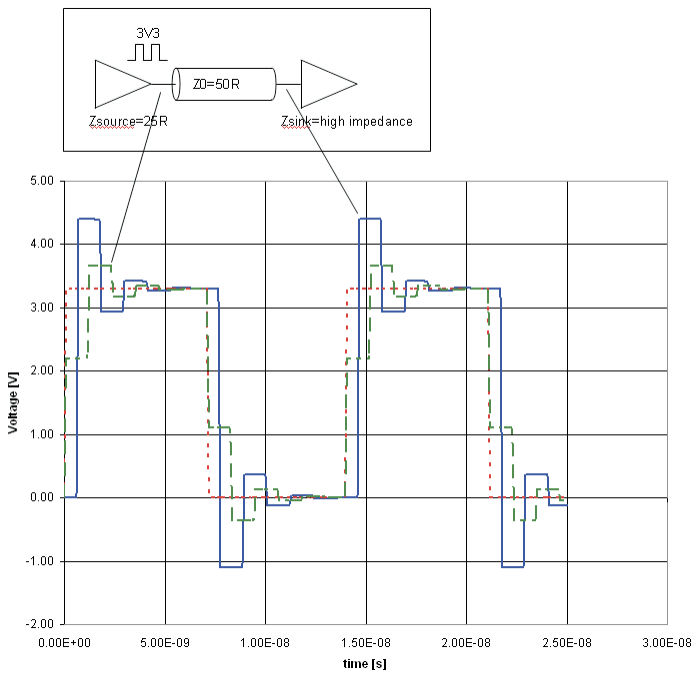
\includegraphics[width=0.4\textwidth]{figures/lythuyet_ringing.png}
                        %     \caption{Minh hoạ hiện tượng ringing do không khớp trở kháng}
                        %     \label{fig:lythuyet_ringing}  
                        % \end{figure}

                        \begin{figure}[H]
                            \centering
                            
                            \begin{minipage}{0.55\textwidth}
                                \paragraph{Signal Integrity (SI)}
                                Signal Integrity là mức độ mà tín hiệu đến đầu nhận vẫn giữ được biên độ, dạng xung và thời điểm chuyển mức như dự kiến. Mất toàn vẹn tín hiệu thể hiện qua hiện tượng méo dạng sóng, overshoot/undershoot, rung (ringing), jitter và gây ra vấn đề lỗi dữ liệu.

                                Các nguyên nhân chính gây suy giảm SI gồm:
                                \begin{itemize}
                                    \item Không khớp trở kháng trên đường truyền.
                                    \item Nhiễu xuyên kênh (crosstalk) giữa các đường mạch gần nhau.
                                    \item Bố trí return path không liên tục, tạo hồi tiếp dòng lớn và tăng cảm kháng.
                                    \item Ảnh hưởng của đặc tính vật liệu PCB như tổn hao điện môi, hiệu ứng bề mặt của dòng điện và hiện tượng tán sắc, gây suy hao biên độ và biến dạng dạng sóng trên các đường truyền dài.
                                \end{itemize}
                            \end{minipage}
                            \hfill
                            \begin{minipage}{0.40\textwidth}
                                \centering
                                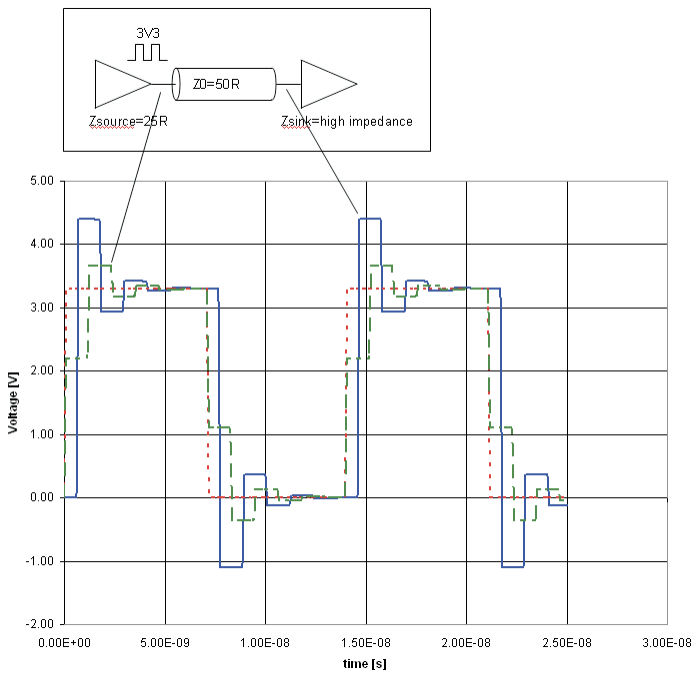
\includegraphics[width=\linewidth]{figures/lythuyet_ringing.png}
                                \caption{Minh hoạ hiện tượng ringing do không khớp trở kháng}
                                \label{fig:lythuyet_ringing}
                            \end{minipage}
                            
                        \end{figure}
                    
                    \paragraph{Return path và vai trò của mặt phẳng tham chiếu}
                        Mỗi tín hiệu tốc độ cao luôn gắn liền với một dòng trở về tương ứng, thường phân bố trên mặt phẳng tham chiếu như ground plane hoặc power plane nằm kề sát lớp tín hiệu. Ở miền tần số cao, dòng trở về có xu hướng tập trung và di chuyển theo đường có tổng trở nhỏ nhất, thông thường là chạy song song và ngay phía dưới đường mạch tín hiệu nhằm giảm diện tích hồi tiếp dòng và cảm kháng. Khi mặt phẳng tham chiếu bị chia cắt, phân mảnh hoặc tồn tại khe hở, đường trở về của dòng tín hiệu sẽ bị gián đoạn và buộc phải đi vòng xa hơn, dẫn đến gia tăng cảm kháng, tăng nhiễu xuyên kênh và phát xạ nhiễu điện từ.

                        % Do đó, trong thiết kế high-speed PCB, việc duy trì một return path liên tục và gần kề với đường tín hiệu là rất quan trọng để đảm bảo tính toàn vẹn tín hiệu. Một số nguyên tắc cơ bản bao gồm:

                        % \begin{itemize}
                        %     \item Định tuyến các tín hiệu tốc độ cao trên những lớp liền kề với một mặt phẳng tham chiếu liên tục để đảm bảo đường trở về ngắn và ổn định.
                        %     \item Tránh cho đường tín hiệu băng qua các khe hở hoặc vùng bị cắt trên mặt phẳng tham chiếu; trong trường hợp bắt buộc phải chuyển lớp, cần bố trí các via mass hoặc via hồi dòng để duy trì tính liên tục của đường trở về.
                        % \end{itemize}
                        
                        % \begin{figure}[H]
                        %     \centering
                        %     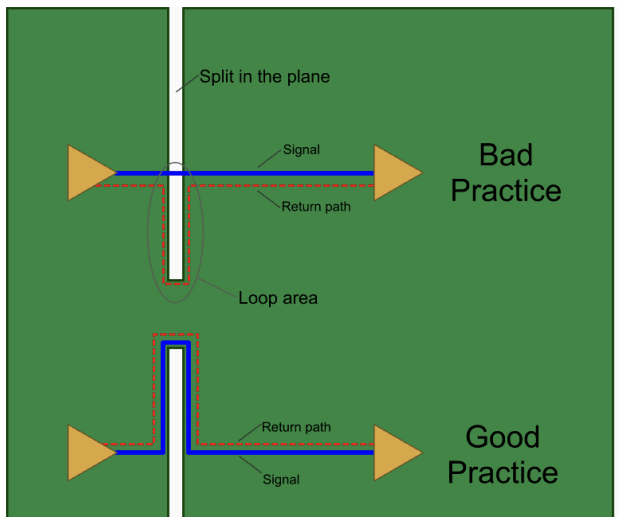
\includegraphics[width=0.4\textwidth]{figures/lythuyet_highspeedlayout.png}
                        %     \caption{Minh hoạ return path liên tục dưới trace trên mặt phẳng tham chiếu}
                        %     \label{fig:sim_highspeedlayout}  
                        % \end{figure}
                        
                        \begin{figure}[H]
                            \centering
                            
                            \begin{minipage}{0.55\textwidth}
                                Do đó, trong thiết kế high-speed PCB, việc duy trì một return path liên tục và gần kề với đường tín hiệu là rất quan trọng để đảm bảo tính toàn vẹn tín hiệu. Một số nguyên tắc cơ bản bao gồm:
                                
                                \begin{itemize}
                                    \item Định tuyến các tín hiệu tốc độ cao trên những lớp liền kề với một mặt phẳng tham chiếu liên tục để đảm bảo đường trở về ngắn và ổn định.
                                    \item Tránh cho đường tín hiệu băng qua các khe hở hoặc vùng bị cắt trên mặt phẳng tham chiếu; trong trường hợp bắt buộc phải chuyển lớp, cần bố trí các via mass hoặc via hồi dòng để duy trì tính liên tục của đường trở về.
                                \end{itemize}
                            \end{minipage}
                            \hfill
                            \begin{minipage}{0.40\textwidth}
                                \centering
                                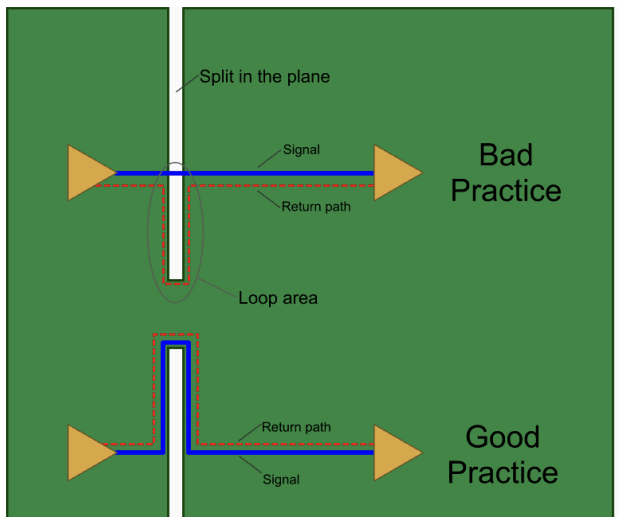
\includegraphics[width=\linewidth]{figures/lythuyet_highspeedlayout.png}
                                \caption{Minh hoạ return path liên tục dưới trace trên mặt phẳng tham chiếu}
                                \label{fig:sim_highspeedlayout}
                            \end{minipage}
                            
                        \end{figure}

                        \paragraph{Hiện tượng phản xạ tín hiệu}
                        
                        Khi tín hiệu lan truyền trên đường truyền có trở kháng đặc trưng \(Z_0\) và gặp một điểm có trở kháng tải \(Z_L\), một phần năng lượng bị phản xạ ngược về nguồn, gây méo dạng sóng và có thể tạo rung. Hệ số phản xạ được cho bởi:
                        \[
                        \Gamma = \frac{Z_L - Z_0}{Z_L + Z_0}
                        \]
                        
                        Giá trị \(\Gamma\) càng xa 0, biên độ sóng phản xạ càng lớn. Điều này là lý do cốt lõi phải kiểm soát và thực hiện phối hợp trở kháng trong thiết kế high-speed.
                        
                        % Trong các hệ thống số tốc độ cao hiện đại, phần lớn các linh kiện giao tiếp như PHY Ethernet, bộ thu phát USB, HDMI/DisplayPort, DDR PHY, các transceiver MIPI hay các bộ chuyển đổi ADC/DAC tốc độ cao đều được thiết kế với trở kháng vào và ra danh định, tương thích với các giá trị trở kháng chuẩn của đường truyền trên PCB và cáp kết nối. Các mức trở kháng này đã được tiêu chuẩn hóa nhằm đảm bảo khả năng truyền dẫn ổn định và tính tương thích giữa các thiết bị. Những giá trị thường gặp bao gồm 50~\(\Omega\) cho các đường tín hiệu single-ended trong nhiều ứng dụng RF và high-speed, 90~\(\Omega\) vi sai cho các giao thức như USB, HDMI, MIPI, và 100~\(\Omega\) vi sai cho Ethernet cũng như nhiều giao thức truyền vi sai khác.

                        % Khi các đường mạch trên PCB không được thiết kế để có trở kháng đặc trưng phù hợp với giá trị mà linh kiện và chuẩn giao thức yêu cầu, sự không khớp trở kháng sẽ xuất hiện tại các điểm chuyển tiếp giữa chip, đường truyền và tải. Hiện tượng này làm tăng hệ số phản xạ \(\Gamma\), dẫn đến các vấn đề như overshoot, ringing, méo dạng sườn tín hiệu, suy giảm biên độ và sai lệch thời điểm lấy mẫu tại phía thu. Do đó, trong thiết kế PCB tốc độ cao, các đường truyền tín hiệu luôn được thiết kế theo nguyên tắc kiểm soát trở kháng (controlled impedance) với các giá trị chuẩn như 50~\(\Omega\), 90~\(\Omega\), 100~\(\Omega\), \ldots nhằm khai thác tối đa đặc tính trở kháng đã được chuẩn hóa.        
                        
                        Trong các hệ thống số tốc độ cao, nhiều linh kiện giao tiếp như Ethernet PHY, USB, HDMI, DDR, MIPI hay ADC/DAC tốc độ cao đều được thiết kế với trở kháng chuẩn nhằm đảm bảo truyền dẫn ổn định và tương thích hệ thống. Các giá trị phổ biến gồm 50~\(\Omega\) cho tín hiệu single-ended, 90~\(\Omega\) vi sai cho USB, HDMI, MIPI, và 100~\(\Omega\) vi sai cho Ethernet cùng các giao thức tương tự.

                        Nếu trở kháng đường truyền trên PCB không phù hợp với yêu cầu của linh kiện hoặc chuẩn giao tiếp, hiện tượng không khớp trở kháng sẽ làm tăng hệ số phản xạ \(\Gamma\), gây overshoot, ringing, méo tín hiệu, suy giảm biên độ và sai lệch thời điểm lấy mẫu. Vì vậy, các đường high-speed thường được thiết kế theo nguyên tắc \textit{controlled impedance} với các mức chuẩn như 50~\(\Omega\), 90~\(\Omega\), 100~\(\Omega\), \ldots nhằm khai thác tối đa đặc tính trở kháng đã được chuẩn hóa.
                    
                \subsubsection{Kiểm soát trở kháng}
                    \paragraph{Trở kháng đặc trưng và các chuẩn thông dụng}
                        Trở kháng đặc trưng \(Z_0\) của đường truyền trên PCB là một đại lượng phân bố liên tục dọc theo chiều dài đường mạch, phản ánh mối quan hệ giữa điện áp và dòng điện của sóng lan truyền trên đường dẫn. Giá trị này phụ thuộc trực tiếp vào hình học của trace như chiều rộng, độ dày đồng, khoảng cách tới mặt phẳng tham chiếu, cấu hình đường truyền (microstrip hoặc stripline), cũng như các thông số điện môi của stack-up PCB. Để tín hiệu tốc độ cao lan truyền ổn định và hạn chế phản xạ, trở kháng đặc trưng cần được duy trì đồng đều trên toàn bộ chiều dài đường truyền, bao gồm cả các đoạn chuyển tiếp như via hoặc vùng breakout linh kiện.

                        Trong thực tế, các giá trị trở kháng mục tiêu đã được chuẩn hóa theo từng giao thức truyền thông và loại đường dẫn nhằm đảm bảo khả năng tương thích giữa linh kiện phát–thu, đường mạch PCB và cáp kết nối. Một số chuẩn trở kháng phổ biến thường được áp dụng trong thiết kế PCB tốc độ cao được liệt kê trong Bảng~\ref{tab:impedance_standards}.
                        
                        \begin{longtable}{|l|c|c|}
                            \caption{Các giá trị trở kháng đặc trưng theo các chuẩn giao thức truyền thông phổ biến.}
                            \label{tab:impedance_standards} \\
                            \hline
                            Giao thức/Chuẩn & Loại đường truyền & Trở kháng mục tiêu \\
                            \hline
                            \endfirsthead
                        
                            \hline
                            Giao thức/Chuẩn & Loại đường truyền & Trở kháng mục tiêu \\
                            \hline
                            \endhead
                        
                            \hline
                            \endfoot
                        
                            \hline
                            \endlastfoot
                        
                            RF, tín hiệu high-speed tổng quát & Single-ended & 50~\(\Omega\) \\
                            USB~2.0/3.x, HDMI & Differential & 90~\(\Omega\) \\
                            Ethernet (10/100/1000/10G) & Differential & 100~\(\Omega\) \\
                            PCIe, DDR3/DDR4 & Differential & 100~\(\Omega\) \\
                            CAN bus, RS-485 & Differential & 120~\(\Omega\) \\
                            LVDS & Differential & 100~\(\Omega\) \\
                            SATA & Differential & 100~\(\Omega\) \\
                        \end{longtable}
                        
                        Mỗi chuẩn giao thức đều quy định chặt chẽ giá trị trở kháng danh định và dung sai cho phép nhằm đảm bảo đặc tính truyền dẫn và khả năng liên thông giữa các thiết bị. Chẳng hạn, các PHY Ethernet thường yêu cầu cặp đường vi sai có trở kháng 100~\(\Omega\) với dung sai khoảng \(\pm 10\%\), trong khi các bộ điều khiển USB được thiết kế để hoạt động tối ưu với đường truyền vi sai 90~\(\Omega\) từ phía phát đến phía thu. Việc tuân thủ đúng các giá trị trở kháng này là điều kiện tiên quyết để giảm phản xạ, hạn chế méo tín hiệu và đảm bảo độ tin cậy của hệ thống truyền thông tốc độ cao.
                    
                    \paragraph{Các yếu tố quyết định trở kháng của đường dây}
                        Trở kháng đặc trưng \(Z_0\) của đường truyền microstrip (trace đặt trên bề mặt PCB) và stripline (trace nằm kẹp giữa hai mặt phẳng tham chiếu) được xác định từ các bài toán trường điện từ phân bố, trong đó điện trường và từ trường lan truyền trong môi trường điện môi xung quanh trace. Mặc dù các công thức chính xác tương đối phức tạp, giá trị \(Z_0\) có thể được phân tích định tính thông qua một số yếu tố chi phối chính sau đây:

                        \begin{enumerate}
                            \item Hằng số điện môi \(\varepsilon_r\): Là tham số đặc trưng của vật liệu PCB, có quan hệ tỷ lệ nghịch với trở kháng đặc trưng. Vật liệu FR4 thông dụng có \(\varepsilon_r\) vào khoảng 4.2–4.6, trong khi các vật liệu chuyên dụng cho tốc độ cao như Rogers RO4000 có \(\varepsilon_r\) thấp hơn, khoảng 3.3–3.5, cho phép đạt cùng giá trị \(Z_0\) với trace rộng hơn và suy hao thấp hơn.
                            \item Độ dày điện môi \(H\): Là khoảng cách từ trace đến mặt phẳng tham chiếu gần nhất, có quan hệ tỷ lệ thuận với \(Z_0\). Với cấu trúc microstrip, \(H\) là khoảng cách từ trace lớp trên đến ground plane phía dưới; với stripline, trace nằm giữa hai plane nên có hai khoảng cách điện môi gần như đối xứng.
                            \item Chiều rộng trace \(W\): Có ảnh hưởng mạnh và tỷ lệ nghịch với \(Z_0\). Khi chiều rộng trace giảm, mật độ điện trường tăng lên và dẫn đến trở kháng đặc trưng cao hơn; ngược lại, trace rộng hơn sẽ làm giảm \(Z_0\).
                            \item Độ dày lớp đồng \(T\): Ảnh hưởng ở mức thứ yếu so với \(W\) và \(H\), thường có quan hệ tỷ lệ nghịch nhẹ với \(Z_0\). Trong thực tế, độ dày đồng phổ biến là 1~oz (khoảng 35~\(\mu\)m) hoặc 0.5~oz (khoảng 17~\(\mu\)m).
                            \item Cấu hình mặt phẳng tham chiếu: Microstrip có ưu điểm dễ chế tạo và dễ định tuyến nhưng chịu ảnh hưởng nhiều hơn từ môi trường bên ngoài và lớp solder mask; stripline được che chắn tốt hơn bởi các plane xung quanh, cho trở kháng ổn định và EMI thấp hơn, nhưng việc định tuyến và kiểm soát stack-up phức tạp hơn.
                            \item Đối với cặp tín hiệu vi sai: Ngoài các yếu tố hình học của từng trace, khoảng cách giữa hai trace \(S\) đóng vai trò quyết định đến mức độ ghép điện dung và điện cảm giữa chúng. Trở kháng vi sai \(Z_{\text{diff}}\) thường được biểu diễn gần đúng theo quan hệ
                            \[
                                Z_{\text{diff}} \approx 2 Z_0 (1 - k),
                            \]
                            trong đó \(k\) là hệ số ghép, phụ thuộc vào khoảng cách \(S\) và cấu trúc stack-up.
                        \end{enumerate}
                        
                        Trong thực tế thiết kế, các tham số hình học và vật liệu hiếm khi được tính toán hoàn toàn bằng tay mà thường được tối ưu hóa thông qua các công cụ field solver tích hợp trong phần mềm thiết kế PCB hoặc công cụ chuyên dụng. Các công cụ này cho phép mô phỏng chính xác trở kháng đặc trưng dựa trên stack-up cụ thể của nhà sản xuất PCB, từ đó đảm bảo sai số nằm trong dung sai cho phép của chuẩn giao tiếp.
                        
                        % Đối với đường microstrip single-ended, một công thức gần đúng thường được sử dụng trong giai đoạn ước lượng ban đầu là:
                        % \[
                        % Z_0 \approx \frac{87}{\sqrt{\varepsilon_r + 1.41}} 
                        % \ln\left(\frac{5.98H}{0.8W + T}\right) \quad (\text{Ohm}),
                        % \]
                        % trong đó \(\varepsilon_r\) là hằng số điện môi của vật liệu, \(H\) là độ dày điện môi, \(W\) là chiều rộng trace và \(T\) là độ dày lớp đồng. Công thức này cho phép đánh giá nhanh xu hướng ảnh hưởng của các tham số hình học trước khi tiến hành mô phỏng chi tiết.

                        % \begin{figure}[H]
                        %     \centering
                        %     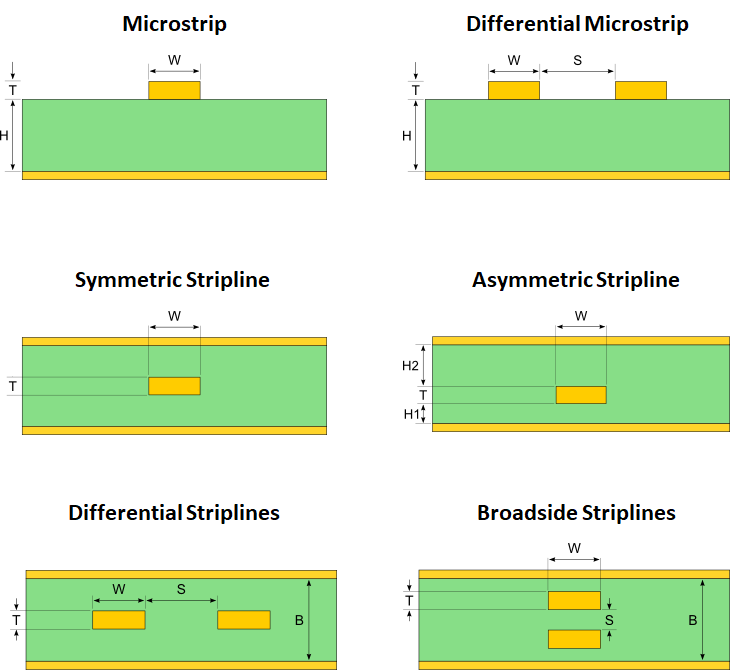
\includegraphics[width=0.4\textwidth]{figures/microstriplines-side-views.png}
                        %     \caption{Minh họa một số cách định tuyến trace trên PCB ảnh hưởng trở kháng}
                        %     \label{fig:microstriplines-side-views}  
                        % \end{figure}

                        \begin{figure}[H]
                            \centering
                            
                            \begin{minipage}{0.55\textwidth}
                                Đối với đường microstrip single-ended, một công thức gần đúng thường được sử dụng trong giai đoạn ước lượng ban đầu là:
                                
                                \[
                                Z_0 \approx \frac{87}{\sqrt{\varepsilon_r + 1.41}} 
                                \ln\left(\frac{5.98H}{0.8W + T}\right) \quad (\text{Ohm}),
                                \]
                                
                                trong đó \(\varepsilon_r\) là hằng số điện môi của vật liệu, \(H\) là độ dày điện môi, \(W\) là chiều rộng trace và \(T\) là độ dày lớp đồng. Công thức này cho phép đánh giá nhanh xu hướng ảnh hưởng của các tham số hình học trước khi tiến hành mô phỏng chi tiết.
                            \end{minipage}
                            \hfill
                            \begin{minipage}{0.40\textwidth}
                                \centering
                                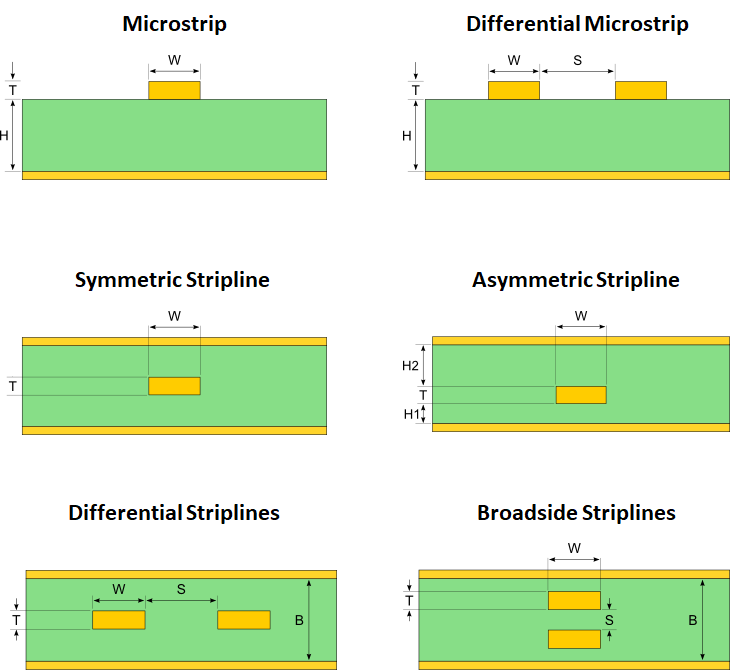
\includegraphics[width=\linewidth]{figures/microstriplines-side-views.png}
                                \caption{Minh họa một số cách định tuyến trace trên PCB ảnh hưởng trở kháng}
                                \label{fig:microstriplines-side-views}
                            \end{minipage}
                            
                        \end{figure}
                        
                    \paragraph{Lý do phải kiểm soát và phối hợp trở kháng}
                        Kiểm soát trở kháng là quá trình thiết kế và chế tạo PCB nhằm đảm bảo trở kháng đặc trưng \(Z_0\) của đường truyền thực tế nằm trong một dải dung sai xác định quanh giá trị mục tiêu, thường ở mức \(\pm 10\%\) hoặc chặt chẽ hơn là \(\pm 5\%\), và được duy trì tương đối đồng đều trên toàn bộ chiều dài đường mạch. Đối với các tín hiệu tốc độ cao, việc kiểm soát này là điều kiện cần để các giả định thiết kế ở mức hệ thống và chuẩn giao tiếp được thỏa mãn trong quá trình vận hành thực tế.
                        
                        % Các mục tiêu chính của việc kiểm soát và phối hợp trở kháng bao gồm:
                        % \begin{itemize}
                        %     \item Giảm thiểu phản xạ tín hiệu: Khi \(Z_0\) của đường truyền được duy trì ổn định và phù hợp với trở kháng của nguồn phát và tải, hệ số phản xạ \(\Gamma\) tiệm cận về 0. Nhờ đó, các hiện tượng như overshoot, ringing và méo dạng tín hiệu được hạn chế, giúp cải thiện biên độ tín hiệu hiệu dụng và chất lượng eye diagram.
                        %     \item Tối ưu hóa quá trình truyền năng lượng tín hiệu: Trong điều kiện trở kháng nguồn, đường truyền và tải được khớp với nhau, năng lượng của xung tín hiệu được truyền đến tải một cách hiệu quả hơn, giảm suy hao do phản xạ và cải thiện độ ổn định của mức logic tại đầu thu.
                        %     \item Đảm bảo tương thích với các chuẩn giao thức tốc độ cao: Nhiều chuẩn truyền thông như USB, Ethernet hay PCIe được xây dựng dựa trên các giả định trở kháng chuẩn hóa. Việc kiểm soát trở kháng đúng giúp duy trì bit error rate thấp, eye diagram mở và đảm bảo các yêu cầu về timing margin theo đặc tả của từng giao thức.
                        % \end{itemize}

                        Các mục tiêu chính của việc kiểm soát và phối hợp trở kháng gồm:
                        \begin{itemize}
                            \item \textbf{Giảm phản xạ tín hiệu:} Khi \(Z_0\) phù hợp với trở kháng nguồn và tải, hệ số phản xạ \(\Gamma\) tiến gần 0, giúp giảm overshoot, ringing và méo dạng tín hiệu.
                            \item \textbf{Tối ưu truyền năng lượng:} Trở kháng được khớp giúp tín hiệu truyền đến tải hiệu quả hơn, giảm suy hao phản xạ và tăng độ ổn định mức logic.
                            \item \textbf{Đáp ứng chuẩn giao tiếp tốc độ cao:} Kiểm soát trở kháng giúp các giao thức như USB, Ethernet, PCIe duy trì bit error rate thấp, eye diagram tốt và đáp ứng timing margin theo đặc tả.
                        \end{itemize}
                                                
                        Trong quá trình sản xuất, nhà chế tạo PCB có thể tinh chỉnh các thông số công nghệ như chiều rộng và khoảng cách trace, cấu trúc stack-up cũng như vật liệu điện môi để đảm bảo trở kháng thực tế của đường truyền nằm trong dải sai số cho phép so với giá trị thiết kế. Việc phối hợp chặt chẽ giữa khâu thiết kế và chế tạo là yếu tố quan trọng để đạt được hiệu quả kiểm soát trở kháng trong các hệ thống PCB tốc độ cao.
                        
                \subsubsection{Quy tắc bố trí để giảm nhiễu, crosstalk và cải thiện EMI}
                    \paragraph{Giảm nhiễu xuyên kênh (crosstalk)}
                        Nhiễu xuyên kênh là hiện tượng nhiễu không mong muốn phát sinh do sự ghép điện dung và ghép cảm ứng giữa các đường tín hiệu đặt gần nhau trên PCB. Trong các hệ thống tốc độ cao, crosstalk có thể làm méo dạng xung, gây jitter, làm thu hẹp eye diagram và trong trường hợp nghiêm trọng có thể dẫn đến lỗi dữ liệu trên các đường tín hiệu lân cận. Mức độ crosstalk phụ thuộc vào khoảng cách giữa các trace, chiều dài đoạn chạy song song, cấu trúc stack-up và chất lượng của đường trở về dòng tín hiệu. 
                        
                        % Một số biện pháp thường được áp dụng để hạn chế crosstalk bao gồm:
                        % \begin{itemize}
                        %     \item Tăng khoảng cách giữa các đường tín hiệu, đặc biệt là giữa các tín hiệu tốc độ cao độc lập; một quy tắc kinh nghiệm phổ biến là duy trì khoảng cách tối thiểu lớn hơn hoặc bằng ba lần chiều cao điện môi đến mặt phẳng tham chiếu hoặc ba lần chiều rộng trace.
                        %     \item Đối với các cặp tín hiệu vi sai, duy trì hai trace chạy song song, sát nhau và có khoảng cách không đổi nhằm tăng cường ghép vi sai, đồng thời làm suy giảm thành phần nhiễu chế độ chung.
                        %     \item Hạn chế các đoạn chạy song song dài giữa tín hiệu nhạy cảm và các tín hiệu có mức nhiễu cao; trong trường hợp các đường buộc phải giao nhau, ưu tiên bố trí vuông góc giữa các lớp khác nhau để giảm ghép điện từ.
                        %     \item Sử dụng mặt phẳng tham chiếu liên tục và đảm bảo đường trở về của dòng tín hiệu ngắn, ổn định nhằm giảm ghép cảm ứng giữa các đường truyền.
                        % \end{itemize}
                        
                        % \begin{figure}[H]
                        %     \centering
                        %     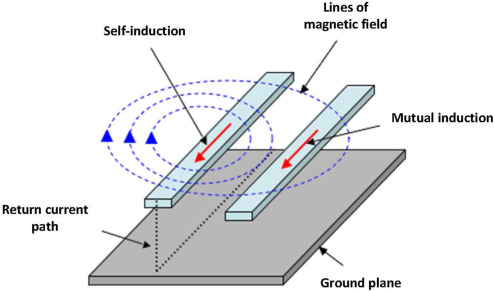
\includegraphics[width=0.4\textwidth]{figures/lythuyet_crosstalk.jpg}
                        %     \caption{Minh họa hiện tượng nhiễu xuyên kênh giữa các đường truyền đặt gần nhau}
                        %     \label{fig:lythuyet_crosstalk}  
                        % \end{figure}

                        \begin{figure}[H]
                            \centering
                            
                            \begin{minipage}{0.55\textwidth}
                                Một số biện pháp hạn chế crosstalk gồm:
                                
                                \begin{itemize}
                                    \item Tăng khoảng cách giữa các trace tín hiệu; quy tắc phổ biến là khoảng cách tối thiểu bằng ba lần chiều rộng trace hoặc chiều cao đến mặt phẳng tham chiếu.
                                    \item Với tín hiệu vi sai, duy trì hai trace song song, khoảng cách cố định để tăng ghép vi sai và giảm nhiễu chế độ chung.
                                    \item Hạn chế các đoạn dài chạy song song giữa tín hiệu nhạy cảm và nguồn nhiễu; nếu bắt buộc giao nhau giữa các lớp, ưu tiên bố trí vuông góc giữa các lớp khác nhau để giảm ghép điện từ.
                                    \item Sử dụng mặt phẳng tham chiếu liên tục để đảm bảo return path ngắn và ổn định, từ đó giảm ghép cảm ứng giữa các đường truyền.
                                \end{itemize}
                            \end{minipage}
                            \hfill
                            \begin{minipage}{0.40\textwidth}
                                \centering
                                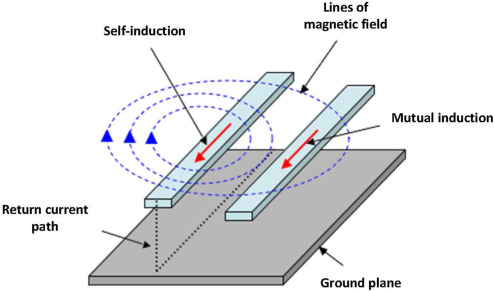
\includegraphics[width=\linewidth]{figures/lythuyet_crosstalk.jpg}
                                \caption{Minh họa hiện tượng nhiễu xuyên kênh giữa các đường truyền đặt gần nhau}
                                \label{fig:lythuyet_crosstalk}
                            \end{minipage}
                            
                        \end{figure}
                    
                    \paragraph{Cải thiện khả năng EMI/EMC}
                        Nhiễu điện từ và khả năng tương thích điện từ là các vấn đề thường gặp trong thiết kế PCB tốc độ cao, do các cạnh tín hiệu nhanh tạo ra phổ tần rộng và dễ phát xạ năng lượng điện từ ra môi trường xung quanh. Layout và routing không hợp lý có thể làm tăng đáng kể mức EMI và ảnh hưởng đến hoạt động của các khối mạch khác trong hệ thống. Để cải thiện đặc tính EMI/EMC, một số nguyên tắc thiết kế high-speed thường được áp dụng như sau:
                        \begin{itemize}
                            \item Giảm diện tích hồi tiếp dòng bằng cách định tuyến tín hiệu ngay trên hoặc sát mặt phẳng tham chiếu liên tục, đồng thời bổ sung via mass khi tín hiệu phải chuyển lớp để duy trì đường trở về liên tục.
                            \item Tránh định tuyến các đường tín hiệu tốc độ cao chạy dọc theo mép PCB trong khoảng dài và không được che chắn; khi cần giảm phát xạ, ưu tiên sử dụng các lớp trong với cấu trúc stripline.
                            \item Hạn chế số lượng via không cần thiết trên các đường high-speed, do via có thể tạo ra gián đoạn trở kháng; đối với PCB dày hoặc tín hiệu tốc độ rất cao, kỹ thuật backdrill có thể được áp dụng để giảm stub của via.
                            \item Phân vùng rõ ràng giữa các miền digital, analog và RF; bố trí các tụ decoupling, tụ bypass và mạch lọc gần chân cấp nguồn của các IC nhạy cảm để giảm nhiễu dẫn.
                        \end{itemize}
                    
                    \paragraph{Một số nguyên tắc layout và routing tiêu biểu cho mạch tốc độ cao}
                        Thiết kế layout và routing cho PCB tốc độ cao cần được xem xét ngay từ giai đoạn đầu của quá trình thiết kế, với các ràng buộc rõ ràng về tín hiệu, lớp mạch và cấu trúc stack-up. Một số nguyên tắc tiêu biểu bao gồm:
                        \begin{itemize}
                            \item Xây dựng cấu trúc stack-up ngay từ đầu, bố trí các lớp tín hiệu xen kẽ với các lớp plane và xác định rõ những lớp dành riêng cho tín hiệu tốc độ cao.
                            \item Áp dụng quy tắc matching độ dài cho các cặp vi sai và các bus song song nhằm giảm lệch thời gian truyền (skew) giữa các đường tín hiệu.
                            \item Tuân thủ nghiêm ngặt các ràng buộc về chiều rộng trace, khoảng cách, lớp định tuyến và cấu trúc via theo yêu cầu của từng giao thức truyền thông cụ thể.
                            \item Tránh các góc gãy 90 độ trên đường tín hiệu tốc độ cao; thay vào đó sử dụng hai góc 45 độ hoặc đường bo cong để giảm gián đoạn trở kháng và hạn chế phát xạ nhiễu.
                        \end{itemize}
                
            \subsection{Power Distribution Network – PDN}
                Mạng phân phối điện (Power Distribution Network – PDN) bao gồm tất cả các kết nối từ Voltage Regulator Module (VRM) đến pad nguồn của chip và lớp kim loại trên die, đảm nhận việc phân phối dòng điện và đường hồi tiếp (return path). PDN bao gồm VRM, tụ khối (bulk decoupling capacitors), via, trace, plane trên PCB, tụ gắn trên board, kết nối package, wire bond / bóng hàn C4, và các kết nối trên chip.
                
                Việc kiểm soát PDN là cực kỳ quan trọng đối với các SoC hiệu năng cao, đặc trưng bởi dòng điện tiêu thụ lớn, điện áp thấp và tần số hoạt động cao. Trở kháng phức tạp của PDN phải được kiểm soát tại pad nguồn của chip. Do dòng tiêu thụ của SoC thường mang dạng sóng vuông (square wave) thay vì tuyến tính, nên sẽ xuất hiện độ gợn (ripple) điện áp do transistor chuyển mạch theo tần số hoạt động. Vì vậy, trở kháng PDN cần được duy trì dưới giá trị trở kháng mục tiêu $Z_{\text{target}}$:
                
                \begin{equation}
                    Z_{\text{target}} = \frac{V_{dd} \times \Delta V_{\text{target}}}{I_{\max}}
                \end{equation}
                
                Trong đó:
                \begin{itemize}
                    \item $V_{dd}$: Điện áp cung cấp (Volt).
                    \item $\Delta V_{\text{target}}$: Điện áp ripple mục tiêu trên rail nguồn (\%).
                    \item $I_{\max}$: Dòng đỉnh lớn nhất trong trường hợp xấu nhất (Amps).
                \end{itemize}
                
                Kiểm soát trở kháng PDN được phân theo các dải tần số khác nhau, mỗi dải chịu ảnh hưởng bởi các thành phần và yêu cầu thiết kế cụ thể:
                
                \begin{itemize}
                    \item \textbf{Dải DC đến kHz:}
                    \begin{itemize}
                        \item Kiểm soát bởi VRM, một số VRM hiện đại phản hồi tới 10–100 kHz.
                        \item Trở kháng tần số thấp được xác định bởi đặc tính của bộ điều chỉnh điện áp (regulator).
                    \end{itemize}
                
                    \item \textbf{Dải kHz đến MHz:}
                    \begin{itemize}
                        \item Kiểm soát bởi tụ khối (bulk capacitors).
                        \item Giá trị tụ được tính dựa trên tần số $f$ mà VRM không còn cung cấp trở kháng thấp:
                        \begin{equation}
                            C = \frac{1}{2\pi f \times Z_{\text{target}}}
                        \end{equation}
                    \end{itemize}
                
                    \item \textbf{Dải MHz đến 100 MHz:}
                    \begin{itemize}
                        \item Kiểm soát bởi tụ ceramic decoupling và PCB plane.
                        \item Chọn lựa tụ decoupling phù hợp và số lượng đủ.
                        \item Khoảng cách via đến pad tụ tối thiểu; đường trả về (return path) ngắn.
                        \item Sử dụng tụ decoupling thấp ESL / cao ESR.
                        \item Khoảng cách giữa lớp power/ground mỏng.
                        \item Trace bề mặt rộng, ngắn từ tụ decoupling đến pin nguồn IC.
                        \item Via đường kính lớn, khoảng cách giữa via nguồn và GND là tối thiểu.
                    \end{itemize}
                
                    \item \textbf{Trên 100 MHz:}
                    \begin{itemize}
                        \item Kiểm soát bởi package IC và tụ trên chip (on-chip capacitance).
                        \item Vượt ngoài khả năng điều khiển từ bên ngoài, được nhà cung cấp IC quản lý thông qua thiết kế package.
                    \end{itemize}
                \end{itemize}
                
                \begin{figure}[H]
                    \centering
                    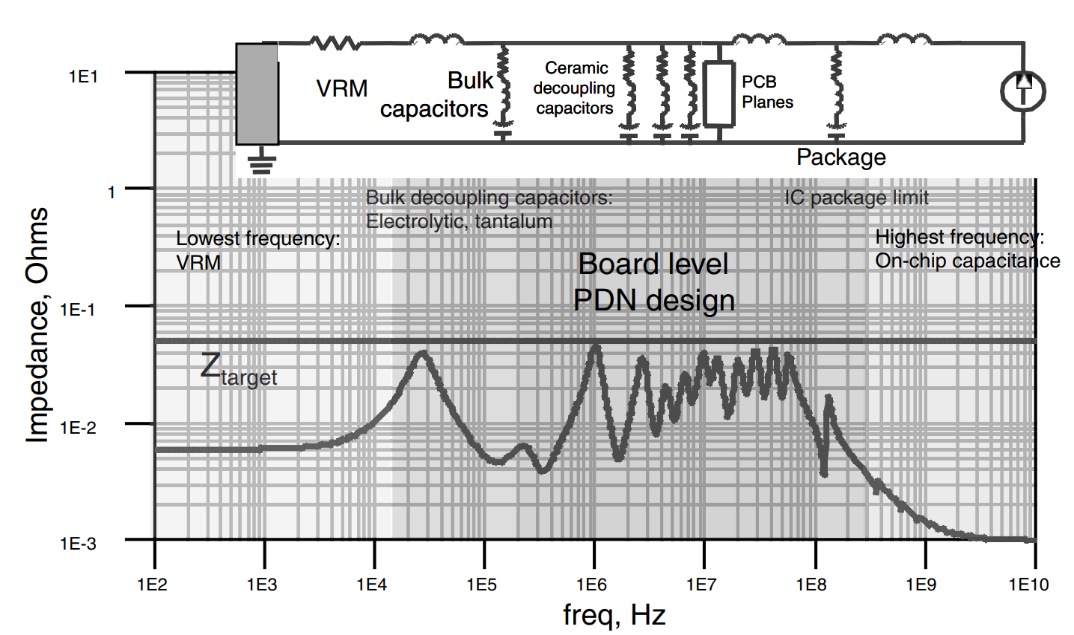
\includegraphics[width=0.7\textwidth]{figures/lythuyet_pdn.png}
                    \caption{Các phần của PDN được phân tách theo dải tần số mà chúng ảnh hưởng}
                    \label{fig:lythuyet_pdn}  
                \end{figure}